\documentclass[a4paper,11pt,UKenglish,twoside,openright]{report}\usepackage[]{graphicx}\usepackage[]{color}
% maxwidth is the original width if it is less than linewidth
% otherwise use linewidth (to make sure the graphics do not exceed the margin)
\makeatletter
\def\maxwidth{ %
  \ifdim\Gin@nat@width>\linewidth
    \linewidth
  \else
    \Gin@nat@width
  \fi
}
\makeatother

\usepackage{Sweavel}



\usepackage{uiothesis}

\title{Identifying School Climate Variables Associated with Students' Financial Literacy Outcomes}
\subtitle{A Cross-Country Comparison\\Using {PISA} 2018 Data}
\author{Tony C. A. Tan}

\begin{document}

% Input faculty etc info
\duoforside[
    fac={Faculty of Educational Sciences},
    dept={Centre for Educational Measurement},
    program={Science (Assessment, Measurement and Evaluation)},
    date={Spring 2021},
%  printer={X-press printing house},
    short
]

% Change page numbering to roman
\pagenumbering{roman}

% Create an acknowledgement page
\thispagestyle{empty}

% This is where I generated the Chinese characters
%//ref http://www.akuziti.com/mb/
% I used font 24.Huawen Xingkai and 100 pixel
\vspace*{\fill}
\begin{figure*}[h]
    
\includegraphics[width=\textwidth]{./Figures/To-parents.png}
\end{figure*}
\begin{flushright}
To my parents
\end{flushright}
\vspace*{\fill}
%\newpage
\clearpage
\thispagestyle{empty}

\vspace*{3cm}

\begin{quote}
    \calligra\huge      % Changes the font to caligraphy and huge size.
\hyphenchar\font=-1     % Stops LaTeX from splitting/hyphenating words
Study hard what interests you the most in the most undisciplined, irreverent and original manner possible.
\end{quote}

\begin{figure*}[h]
    \flushright
    
\includegraphics[width=0.50\textwidth]{./Figures/Feynman-Signature.jpg}
\end{figure*}
\vspace*{-1cm}

%\begin{flushright}
%--- Richard P. Feynman
%\end{flushright}

\setcounter{page}{0}
% End of acknowledgement page

% Put Table of Content here
\tableofcontents

% Put a List of Tables here
\listoftables

% Put a List of Figures here
\listoffigures



% APA7 Rule 2.21 Line Spacing
%\onehalfspacing
\doublespacing

% Acknowledgement

\chapter*{Acknowledgement}
\label{Ac}

Thank-you goes to

% Popular Abstract

\chapter*{Popular Abstract}
\label{Ab.0}

Preparing youth for life-long success with numeracy, literacy and science capability has been the foundation for all schooling. The post-global financial crises and post-COVID era, in addition, imposes increasing demand on financial literacy for school leavers. Since 2012, OECD has been a pioneer in measuring 15-year-olds' financial literacy through its triennial Programme for International Student Assessment (PISA) cycles. Subsequent analyses using PISA data, however, reported paradoxical results that more classroom interventions tend to be associated with either no differences or even lower scores in students' financial literacy measures. It is in educators' interest therefore to carefully examine the relationship between school climate variables, including the academic, safety, community and institutional envrionment aspects of students' lives, and their financial literacy outcomes.

% Abstract

\chapter*{Abstract}
\label{Ab.1}

Repeated economic crises in recent memory have exposed the harsh consequences of financial \emph{illiteracy} shared by high proportions of the general population. Policy makers experienced little resistance when identifying youth as the most effective group for bringing about improvement in citizens' ability to engage with economic and financial matters, but opinions quickly diverge over the optimal approaches for achieving such targeted outcome. Existing literature frequently reports the importance of family environment in cultivating students' financial literacy through the process of ``financial socialisation'' -- [definition goes here] (reference). Such practice, however, encounters interrogation by educators over equity concerns should families remain the main arena for financial literacy development. Schools play vital roles in alleviating inequality in accessing education and training in general but scarce research so far has been devoted into identifying the specific classroom factors that are most effective in advancing students' financial literacy outcomes. The current study therefore attempts to contribute to this enquiry by investigating the relationship between school climate variables and students' financial literacy achievement with an aim of stimulating policy debate about the levers and instruments available to education interventionists for the purpose of improving young people's financial literacy and preparedness as they step into an increasingly uncertain world. Using the 2018 PISA dataset, this paper employs a three-level hierarchical model to conduct cross-country comparisons to highlight school climate variables that are most strongly associated with high financial literacy outcomes.

% End of front matter. None of the pages so far counts towards the page limit.
\clearpage
\thispagestyle{empty}

% Restart page number. Page count starts here.
\pagenumbering{arabic}
\setcounter{page}{0} % Do not swap these two command. Need new chapter to be "Open right".

% Chapter 1 Introduction

\chapter{Introduction}
\label{chp:1}

%\epigraph{If you think education is expensive, try ignorance}{Derek Bok}

%//mark Broad motivation

Repeated economic crises in recent memory have exposed the harsh consequences of financial \emph{illiteracy} shared by high proportions of the general population. Low levels of financial literacy are observed not only in less developed countries such as India and Indonesia \parencite{cole:2009} but also in advanced economies such as the USA \parencite{huston:2012}, Germany \parencite{bucherkoenen:2016} and OECD countries \parencite{lusardi:2015a}. Amongst the many redress schemes aimed at promoting citizens' financial capability, the return on investment is the highest when intervention is applied early in life. \textcite{lusardi:2014} have shown that providing financial knowledge to the least educated before they enter the labour market increases their well-being by approximately 82\% of their initial wealth, while the rate of return is around 56\% for college graduates---results that are significant both statistically and economically.

Research efforts aiming at advancing youth's financial literacy over the years evolved into two strands: on the design and evaluation of school financial education programs, and on the influence of home environment through the process of financial socialisation---the intentional or involuntary transmission of financial concepts which are required to functioning successfully in society \parencite{bowen:2002}. A recent meta-analysis conducted by \textcite{kaiser:2020} found that while school financial education programs had sizeable impacts on \emph{financial knowledge} ($+0.33\ SD$) similar to education interventions in other domains, their effect on students' \emph{financial behaviour} is quite small ($+0.07\ SD$). This conclusion added to a list of weak or non-findings regarding the long-term behavioural effect brought about by school financial education programs. \textcite{brown:2016}, for instance, reported mixed outcome in students' long-term financial well-being depending on the programs received; whereas \textcite{cole:2016} observed that traditional personal finance courses lacked any explanatory power in accounting for graduates' financial outcome once the additional mathematics training in which finance topics were packaged has been controlled for. Despite careful controls and thoughtful study designs, correlating classroom interventions and young people's financial literacy outcomes has repeatedly yielded paradoxical results of non-significant or even negative relationship; any positive findings remain small in magnitudes and/or are sensitive to robust analyses.

Optimism, fortunately, runs higher at the financial socialisation camp. Building on the acknowledgement that families serve as information filters from the outside world \parencite{danes:2007} as well as the foundation for youth's continued financial concept formation, \textcite{gudmunson:2011} put forward a family financial socialisation theory to accommodate both the \emph{process} and the \emph{outcome} for variations in young people's financial capabilities. Using structural equation modelling, \textcite{jorgensen:2010} was able to show that perceived parental influence had a direct and moderately significant influence on financial attitude, did \emph{not} have an effect on \emph{financial knowledge}, and had an indirect and moderately significant influence on financial behaviour, mediated through financial attitude. This attitude(A)--behaviour(B)
--cognition(C) conceptualisation of financial literacy \parencite{potrich:2015} continues to influence subsequent research effort. More recently, \textcite{morenoherrero:2018a} continued this line of enquiry by applying multilevel regression analyses to 2015 PISA data and reported that students' financial literacy was associated mainly with understanding the value of saving and discussing money matters with parents. In addition, exposure and use of financial products, in particular holding a bank account, improved students' financial knowledge as well.

One chief concern for every research project is the quality of its data source. Amongst competing inventories, PISA stands out as a comprehensive and reliable source of data for measuring 15-year-olds' financial literacy outcomes thanks to OECD's careful sampling procedure and attention to construct validity of measurement. Following statistical theory, PISA designers firstly recognise the hierarchical nature of education research data such that students are nested in schools, and schools are further nested in countries. In addition, one student weight is assigned to each observation in order to account for the fact that not all schools in a country are equally likely to be sampled by the PISA organiser; and given a particular school that has been chosen, not every student in this school is equally likely to be asked to participate in the test \parencite{rust:2014}. A third complication arises from the ``planned missingness'' in students' responses because each participant is only given a small number of questions relative to the entire test bank in order to ensure their responses are not undermined by tiredness \parencite{vondavier:2014}, leading to the outcome variables being represented by ten plausible values. Lastly, PISA consulted and synthesised multiple schools of thoughts \parencite{PISAframework} before constructing financial literacy as \blockquote{the knowledge and understanding of financial concepts and risks, and the skills, motivation and confidence to apply such knowledge and understanding in order to make effective decisions across a range of financial contexts, to improve the financial well-being of individuals and society, and to enable participation in economic life. (p. 128)} As a result, 2018 PISA data set \parencite{FLdata} provides not only variables measuring \emph{cognitive} outcomes but also \emph{affective} factors such as familiarity with concepts of finance and confidence about financial matters, enabling a nuanced study design involving decomposing the total effect of financial literacy development into its ``brain'' (cognitive) and ``heart'' (affective) pathways.

% APA7 Rule 6.50 Lettered Lists and 6.51 Numbered Lists
The current study wishes to take advantage of the latest wave of 2018 PISA results and investigate the covariation financial literacy outcomes share with the following four aspects of young people's daily lives, inspired by school climate literature \parencite{wang:2016}:
\begin{enumerate*}[label={(\alph*)}]
    \item academic training, including any financial education programs received at schools;
    \item safety perception about their schools;
    \item financial socialisation experienced at home; and
    \item their schools' resource endowment.
\end{enumerate*}
More specifically, this project aims to answer these three research questions:
\begin{enumerate}
    \item[RQ1.] Having controlled for demographic characteristics such as socio-economic status, sex and immmigration history, to what extent can the variation in students' financial literacy outcomes be accounted for by each of the school climate variables mentioned above.
    \item[RQ2.] How does the total effect each school climate variable carries decompose into cognitive and affect pathways.
    \item[RQ3.] How do these effects differ across countries.
\end{enumerate}

%//mark Definition of key terms

%//mark My topic(s)

%//mark Zoom out: Why is this topic important?

\newpage

%\parencite{abubakar:2020,agarwal:2015,agnew:2015a,agnew:2015b,agyei:2018,akbenselcuk:2014,ali:2014,allgood:2016,amagir:2018,aprea:2015,arceogomez:2017,arellano:2014,arellano:2018,arthur:2012,atkinson:2011,bartholomae:2016,batsaikhan:2018,becchetti:2013,beckmann:2020,behrman:2012,bel:2015,belas:2016,bernheim:2001,birbili:2015,blue:2014a,blue:2014b,blue:2017,blue:2018,blue:2020,boisclair:2017,bongini:2012,bover:2018,bover:2020,bowen:2002,bray:1995,breitbach:2016,brimble:2013,brown:2013,brown:2016,brown:2018,bucciol:2020,bucherkoenen:2016,caliendo:2013,cameron:2013,campioni:2017,carlin:2012a,carlin:2012b,carvalho:2020,chambers:2018,chambers:2019,chatfield:1978,chen:2018,chiang:2020,ciemleja:2014a,ciemleja:2014b,cole:2009,cole:2016,collins:2013,connolly:2015,cordero:2019,cude:2016,cupak;2018b,cupak:2018a,cupak:2018c,curugan:2020,danes:2007,davies:2016,davoli:2020,debeckker:2019,debeckker:2020,driva:2016,eickelmann:2016,emmons:2005,eniola:2016,erner:2016,ethics,fabris:2016,farinella:2017,fernandes:2014,ferrari:2019,FLdata,fonseca:2012,fornero:2019,forster:2017,fraczek:2015,frisancho:2019,garder:1985,garg:2018,geiger:2016,gomes:2020,goyal:2020,gramatki:2017,grohmann:2015,grohmann:2016,grohmann:2018,gudmunson:2011,gudmunson:2016,guest:2018,hanushek:2012a,hanushek:2012b,happ:2016,hastings:2013,hdr:data,henderson:2020,hira:2016,ho:2020,holtsch:2016,huston:2010,huston:2012,ibarra:2019,intsvy,janssen:2019,jappelli:2010,jappelli:2013,jappelli:2015,jorgensen:2010,jüttler:2016,kaiser:2020,kalmi:2018,karakurumozdemir:2019,kell:2014,kenayathulla:2020,khalil:2020,khan:2017,khoirunnisaa:2020,kiliyanni:2016,kim:2020,klapper:2019,klieme:2020,kosor:2020,kunovskaya:2014,laukaityte:2018,leumann:2016,li:2020,liaqat:2020,longobardi:2017,longobardi:2018,loprete:2013,lusardi:2007,lusardi:2008,lusardi:2010,lusardi:2011,lusardi:2012,lusardi:2013,lusardi:2014,lusardi:2015a,lusardi:2015b,lusardi:2016,lusardi:2017,lusardi:2019a,lusardi:2019b,mancebon:2015,mancebon:2019,mandell:2009,mandmaa:2020,marsh:2004,marsh:2012,marsh:2019,matheson:2020,mitchell:2015,mohammadpour:2013,morenoherrero:2018a,morenoherrero:2018b,mountain:2020,norvilitis:2006,norvilitis:2010,nurhasanah:2020,oberrauch:2019,oecd:2005,oecd:2009,olivermarquez:2020,opletalova:2015,page:2020,paolostella:2020,pesando:2018,peugh:2010,pinto:2011,pinto:2012,pinto:2013,pokropek:2016,potrich:2015,potrich:2016,preston:2019,R,remund:2010,riitsalu:2016,rinaldi:2012,rodriguez:2020,rohatgi:2020,rubin:1987,rust:2014,rustomfram:2015,rutkowski:2010,savard:2020a,sawatzki:2020,schmeiser:2013,schuhen:2014,schurkmann:2013,sellar:2013,serido:2016,shadish:2002,shen:2016,shim:2009,shim:2010,siegfried:2016,silgoner:2015,skagerlund:2018,soderlund:2020,sole:2014,spataro:2017,stanisavjevic:2018,stolper:2017,strahija:2020,strietholt:2018,sun:2012,sutter:2020,taylor:2013,tchatoka:2020,teenharari:2016,tezel:2015,thomas:2018,thomson:2017,titko:2015a,titko:2015b,toosi:2020,vale:2020,vancampenhout:2015,vanrooij:2011,vondavier:2014,vyvyan:2014,wang:2015,wang:2020,wastad:2016,willis:2008,worldbank:data,young:2013,young:2015,youshino:2015,zhu:2012,zhu:2015,zokaityte:2016,utkarsh:2020,grund:2020,guttman:1944,goodman:1975,green:1956,ozkale:2020a,endsley:2020,indefenso:2020,erylmaz:2020,wuttke:2020,ozkale:2020b,bottazzi:2020,ruoss:2020,runge:2020,warm:1989,vanwee:2016,savard:2020b,williams:2020,stride:2015,caoalvira:2020}

% Chapter 2 Theoretical framework

\chapter{Conceptual Framework}
\label{chp:2}

\section{In-depth definitions of ``financial literacy''}

\subsection{Every term my readers need in order to understand my research question}

\subsection{Survey not only PISA but also alternative definitions, even critiques of such definitions}

\subsection{Any practices that are common in maths/literature but uncommon in financial literacy? Meaning? Implies?}

\newpage

\section{Country-level Financial Knowledge Index}

PISA 2018 financial literacy dataset \parencite{FLdata} provides rich information about students and schools. For the purpose of cross-country comparison, however, the country-level financial literacy information must be addressed separately by the researchers. Earlier attempts such as \textcite{morenoherrero:2018a} approximated this information using a variable ``quality of math and science education'' to control for country-level differences since consensus is yet to emerge about the most appropriate measure for countries' financial knowledge. Inspired by the UN's approach to forming Human Development Indices, a recent publication by \textcite{olivermarquez:2020} proposed a macroeconomic measure for countries' general financial knowledge levels by examining their economic capability, educational training, existing practices in the financial markets as well as incentives to interact with financial products. More specifically, the authors considered a country's economic capability, represented by its GDP per capita, to be a key dimension in bringing about its financial knowledge index (FKI). Secondly, literature converges on the importance of educational training for a country's financial knowledge capability \parencite{oecd:2005}. Thirdly, countries with regular engagement with sophisticated financial products and financial markets should possess higher FKI. Lastly, countries with higher aggregate consumption levels and with ageing populations are likely to possess higher FKI due to more frequent exposure and pressure in retirement provision, respetively. Macroeconomic data needed for these computations can be sourced from the World Bank \parencite{worldbank:data} and the United Nations' \textit{Human Development Reports} \parencite{hdr:data}.

Combining individual and institutional data cources can be a productive approach in international large-scale assessment (ILSA) research. According to the framework for comparative education analyses \parencite{bray:1995}, this project extends education outcome measures to a country level, addresses the aspect of society and labour market, and relates countries' entire populations to ILSA research \parencite{strietholt:2018}. By combining education outcome data with countries' economic performance indicators, this project remains most comparable to \textcite{hanushek:2012a}---while these authors looked into the relationship between countries' education achievement and their GDP growth, the current investigation highlights how countries' GDP, along with other macroeconomic practices, in turn systematically impacts on their youth's educational performance.

\newpage

% Table generated by Excel2LaTeX from sheet 'Sheet2'
\ltable{tab:Missing}{Percentages of Missing Values}{
      \begin{tabular}{ccrrrrrrrrrrrrrrrrrrrr}
      \toprule
      CNT   &       & \multicolumn{1}{c}{\rotatebox{90}{\texttt{MALE}}} & \multicolumn{1}{c}{\rotatebox{90}{\texttt{IMMI1GEN}}} & \multicolumn{1}{c}{\rotatebox{90}{\texttt{IMMI2GEN}}} & \multicolumn{1}{c}{\rotatebox{90}{\texttt{ESCS}}} & \multicolumn{1}{c}{\rotatebox{90}{\texttt{FCFMLRTY}}} & \multicolumn{1}{c}{\rotatebox{90}{\texttt{FLCONFIN}}} & \multicolumn{1}{c}{\rotatebox{90}{\texttt{PERFEED}}} & \multicolumn{1}{c}{\rotatebox{90}{\texttt{TEACHINT}}} & \multicolumn{1}{c}{\rotatebox{90}{\texttt{FLSCHOOL}}} & \multicolumn{1}{c}{\rotatebox{90}{\texttt{DISCRIM}$^\dagger$}} & \multicolumn{1}{c}{\rotatebox{90}{\texttt{BELONG}}} & \multicolumn{1}{c}{\rotatebox{90}{\texttt{BULLY}}} & \multicolumn{1}{c}{\rotatebox{90}{\texttt{FLFAMILY}}} & \multicolumn{1}{c}{\rotatebox{90}{\texttt{CURSUPP}$^\dagger$}} & \multicolumn{1}{c}{\rotatebox{90}{\texttt{PASCHPOL}$^\dagger$}} & \multicolumn{1}{c}{\rotatebox{90}{\texttt{W\_SCH}}} & \multicolumn{1}{c}{\rotatebox{90}{\texttt{PRIVATE}}} & \multicolumn{1}{c}{\rotatebox{90}{\texttt{STRATIO}}} & \multicolumn{1}{c}{\rotatebox{90}{\texttt{EDUST}}} & \multicolumn{1}{c}{\rotatebox{90}{\texttt{STAFFST}}} \\
      \midrule
      BGR$^\dagger$   &       & 0     & \cellcolor[rgb]{ 1,  .945,  .945}6 & \cellcolor[rgb]{ 1,  .945,  .945}6 & \cellcolor[rgb]{ 1,  .973,  .973}3 & \cellcolor[rgb]{ 1,  .882,  .882}12 & \cellcolor[rgb]{ 1,  .733,  .733}27 & \cellcolor[rgb]{ 1,  .898,  .898}10 & \cellcolor[rgb]{ 1,  .906,  .906}10 & \cellcolor[rgb]{ 1,  .792,  .792}21 & \cellcolor[rgb]{ 1,  .722,  .722}28 & \cellcolor[rgb]{ 1,  .808,  .808}19 & \cellcolor[rgb]{ 1,  .694,  .694}31 & \cellcolor[rgb]{ 1,  .784,  .784}22 & \cellcolor[rgb]{ 1,  0,  0}100 & \cellcolor[rgb]{ 1,  0,  0}100 & 0     & \cellcolor[rgb]{ 1,  0,  0}100 & \cellcolor[rgb]{ 1,  .922,  .922}8 & \cellcolor[rgb]{ 1,  .973,  .973}3 & \cellcolor[rgb]{ 1,  .973,  .973}3 \\
      BRA   &       & 0     & \cellcolor[rgb]{ 1,  .949,  .949}5 & \cellcolor[rgb]{ 1,  .949,  .949}5 & \cellcolor[rgb]{ 1,  .98,  .98}2 & \cellcolor[rgb]{ 1,  .878,  .878}12 & \cellcolor[rgb]{ 1,  .667,  .667}34 & \cellcolor[rgb]{ 1,  .91,  .91}9 & \cellcolor[rgb]{ 1,  .925,  .925}8 & \cellcolor[rgb]{ 1,  .796,  .796}21 & \cellcolor[rgb]{ 1,  .643,  .643}36 & \cellcolor[rgb]{ 1,  .776,  .776}23 & \cellcolor[rgb]{ 1,  .6,  .6}40 & \cellcolor[rgb]{ 1,  .765,  .765}24 & \cellcolor[rgb]{ 1,  .831,  .831}17 & \cellcolor[rgb]{ 1,  .816,  .816}19 & 0     & 0     & \cellcolor[rgb]{ 1,  .882,  .882}12 & \cellcolor[rgb]{ 1,  .941,  .941}6 & \cellcolor[rgb]{ 1,  .933,  .933}7 \\
      CAN$^\dagger$   &       & 0     & \cellcolor[rgb]{ 1,  .933,  .933}7 & \cellcolor[rgb]{ 1,  .933,  .933}7 & \cellcolor[rgb]{ 1,  .953,  .953}5 & \cellcolor[rgb]{ 1,  .894,  .894}11 & \cellcolor[rgb]{ 1,  .851,  .851}15 & \cellcolor[rgb]{ 1,  0,  0}100 & \cellcolor[rgb]{ 1,  0,  0}100 & \cellcolor[rgb]{ 1,  .875,  .875}13 & \cellcolor[rgb]{ 1,  0,  0}100 & \cellcolor[rgb]{ 1,  .925,  .925}8 & \cellcolor[rgb]{ 1,  .859,  .859}14 & \cellcolor[rgb]{ 1,  .867,  .867}14 & \cellcolor[rgb]{ 1,  0,  0}100 & \cellcolor[rgb]{ 1,  0,  0}100 & 0     & 0     & \cellcolor[rgb]{ 1,  0,  0}100 & \cellcolor[rgb]{ 1,  .988,  .988}2 & \cellcolor[rgb]{ 1,  .984,  .984}2 \\
      CHL   &       & 0     & \cellcolor[rgb]{ 1,  .961,  .961}4 & \cellcolor[rgb]{ 1,  .961,  .961}4 & \cellcolor[rgb]{ 1,  .976,  .976}3 & \cellcolor[rgb]{ 1,  .906,  .906}10 & \cellcolor[rgb]{ 1,  .769,  .769}24 & \cellcolor[rgb]{ 1,  .953,  .953}5 & \cellcolor[rgb]{ 1,  .961,  .961}4 & \cellcolor[rgb]{ 1,  .875,  .875}13 & \cellcolor[rgb]{ 1,  .706,  .706}30 & \cellcolor[rgb]{ 1,  .851,  .851}15 & \cellcolor[rgb]{ 1,  .663,  .663}34 & \cellcolor[rgb]{ 1,  .855,  .855}15 & \cellcolor[rgb]{ 1,  .918,  .918}9 & \cellcolor[rgb]{ 1,  .918,  .918}8 & 0     & 0     & \cellcolor[rgb]{ 1,  .82,  .82}18 & \cellcolor[rgb]{ 1,  .906,  .906}9 & \cellcolor[rgb]{ 1,  .914,  .914}9 \\
      ESP   &       & 0     & \cellcolor[rgb]{ 1,  .973,  .973}3 & \cellcolor[rgb]{ 1,  .973,  .973}3 & \cellcolor[rgb]{ 1,  .984,  .984}2 & \cellcolor[rgb]{ 1,  .957,  .957}5 & \cellcolor[rgb]{ 1,  .792,  .792}21 & \cellcolor[rgb]{ 1,  .973,  .973}3 & \cellcolor[rgb]{ 1,  .98,  .98}2 & \cellcolor[rgb]{ 1,  .929,  .929}7 & \cellcolor[rgb]{ 1,  .757,  .757}25 & \cellcolor[rgb]{ 1,  .91,  .91}9 & \cellcolor[rgb]{ 1,  .718,  .718}29 & \cellcolor[rgb]{ 1,  .918,  .918}8 & \cellcolor[rgb]{ 1,  0,  0}100 & \cellcolor[rgb]{ 1,  0,  0}100 & 0     & 0     & \cellcolor[rgb]{ 1,  .89,  .89}11 & \cellcolor[rgb]{ 1,  .949,  .949}5 & \cellcolor[rgb]{ 1,  .945,  .945}6 \\
      EST   &       & 0     & \cellcolor[rgb]{ 1,  .969,  .969}3 & \cellcolor[rgb]{ 1,  .969,  .969}3 & \cellcolor[rgb]{ 1,  .976,  .976}3 & \cellcolor[rgb]{ 1,  .957,  .957}4 & \cellcolor[rgb]{ 1,  .925,  .925}8 & \cellcolor[rgb]{ 1,  .969,  .969}3 & \cellcolor[rgb]{ 1,  .973,  .973}3 & \cellcolor[rgb]{ 1,  .945,  .945}6 & \cellcolor[rgb]{ 1,  .914,  .914}9 & \cellcolor[rgb]{ 1,  .957,  .957}5 & \cellcolor[rgb]{ 1,  .898,  .898}11 & \cellcolor[rgb]{ 1,  .941,  .941}6 & \cellcolor[rgb]{ 1,  0,  0}100 & \cellcolor[rgb]{ 1,  0,  0}100 & 0     & 0     & 0     & 0     & 0 \\
      FIN$^\dagger$   &       & 0     & \cellcolor[rgb]{ 1,  .98,  .98}2 & \cellcolor[rgb]{ 1,  .98,  .98}2 & \cellcolor[rgb]{ 1,  .984,  .984}2 & \cellcolor[rgb]{ 1,  .957,  .957}4 & \cellcolor[rgb]{ 1,  .898,  .898}10 & \cellcolor[rgb]{ 1,  .973,  .973}3 & \cellcolor[rgb]{ 1,  .973,  .973}3 & \cellcolor[rgb]{ 1,  .937,  .937}6 & \cellcolor[rgb]{ 1,  0,  0}100 & \cellcolor[rgb]{ 1,  .937,  .937}6 & \cellcolor[rgb]{ 1,  .894,  .894}11 & \cellcolor[rgb]{ 1,  .933,  .933}7 & \cellcolor[rgb]{ 1,  0,  0}100 & \cellcolor[rgb]{ 1,  0,  0}100 & 0     & \cellcolor[rgb]{ 1,  0,  0}100 & \cellcolor[rgb]{ 1,  .98,  .98}2 & \cellcolor[rgb]{ 1,  .925,  .925}7 & \cellcolor[rgb]{ 1,  .925,  .925}7 \\
      GEO   &       & 0     & \cellcolor[rgb]{ 1,  .949,  .949}5 & \cellcolor[rgb]{ 1,  .949,  .949}5 & \cellcolor[rgb]{ 1,  .984,  .984}2 & \cellcolor[rgb]{ 1,  .914,  .914}9 & \cellcolor[rgb]{ 1,  .737,  .737}26 & \cellcolor[rgb]{ 1,  .906,  .906}9 & \cellcolor[rgb]{ 1,  .914,  .914}9 & \cellcolor[rgb]{ 1,  .827,  .827}17 & \cellcolor[rgb]{ 1,  0,  0}100 & \cellcolor[rgb]{ 1,  .855,  .855}15 & \cellcolor[rgb]{ 1,  .784,  .784}22 & \cellcolor[rgb]{ 1,  .796,  .796}21 & \cellcolor[rgb]{ 1,  .965,  .965}4 & \cellcolor[rgb]{ 1,  .953,  .953}5 & 0     & 0     & \cellcolor[rgb]{ 1,  .988,  .988}1 & \cellcolor[rgb]{ 1,  .984,  .984}2 & \cellcolor[rgb]{ 1,  .98,  .98}2 \\
      IDN   &       & 0     & \cellcolor[rgb]{ 1,  .976,  .976}3 & \cellcolor[rgb]{ 1,  .976,  .976}3 & \cellcolor[rgb]{ 1,  .996,  .996}1 & \cellcolor[rgb]{ 1,  .969,  .969}3 & \cellcolor[rgb]{ 1,  .945,  .945}6 & \cellcolor[rgb]{ 1,  .973,  .973}3 & \cellcolor[rgb]{ 1,  .98,  .98}2 & \cellcolor[rgb]{ 1,  .953,  .953}5 & \cellcolor[rgb]{ 1,  .969,  .969}3 & \cellcolor[rgb]{ 1,  .976,  .976}2 & \cellcolor[rgb]{ 1,  .949,  .949}5 & \cellcolor[rgb]{ 1,  .949,  .949}5 & \cellcolor[rgb]{ 1,  0,  0}100 & \cellcolor[rgb]{ 1,  0,  0}100 & 0     & 0     & \cellcolor[rgb]{ 1,  .773,  .773}23 & \cellcolor[rgb]{ 1,  .863,  .863}14 & \cellcolor[rgb]{ 1,  .863,  .863}14 \\
      ITA   &       & 0     & \cellcolor[rgb]{ 1,  .965,  .965}4 & \cellcolor[rgb]{ 1,  .965,  .965}4 & \cellcolor[rgb]{ 1,  .976,  .976}3 & \cellcolor[rgb]{ 1,  .933,  .933}7 & \cellcolor[rgb]{ 1,  .827,  .827}17 & \cellcolor[rgb]{ 1,  .957,  .957}4 & \cellcolor[rgb]{ 1,  .961,  .961}4 & \cellcolor[rgb]{ 1,  .902,  .902}10 & \cellcolor[rgb]{ 1,  .769,  .769}23 & \cellcolor[rgb]{ 1,  .902,  .902}10 & \cellcolor[rgb]{ 1,  .733,  .733}27 & \cellcolor[rgb]{ 1,  .882,  .882}12 & \cellcolor[rgb]{ 1,  .847,  .847}16 & \cellcolor[rgb]{ 1,  .835,  .835}17 & 0     & 0     & \cellcolor[rgb]{ 1,  .906,  .906}9 & \cellcolor[rgb]{ 1,  .969,  .969}3 & \cellcolor[rgb]{ 1,  .973,  .973}3 \\
      LTU   &       & 0     & \cellcolor[rgb]{ 1,  .976,  .976}3 & \cellcolor[rgb]{ 1,  .976,  .976}3 & \cellcolor[rgb]{ 1,  .973,  .973}3 & \cellcolor[rgb]{ 1,  .961,  .961}4 & \cellcolor[rgb]{ 1,  .882,  .882}12 & \cellcolor[rgb]{ 1,  .973,  .973}3 & \cellcolor[rgb]{ 1,  .976,  .976}3 & \cellcolor[rgb]{ 1,  .949,  .949}5 & \cellcolor[rgb]{ 1,  .831,  .831}17 & \cellcolor[rgb]{ 1,  .925,  .925}8 & \cellcolor[rgb]{ 1,  .8,  .8}20 & \cellcolor[rgb]{ 1,  .937,  .937}7 & \cellcolor[rgb]{ 1,  0,  0}100 & \cellcolor[rgb]{ 1,  0,  0}100 & 0     & 0     & 0     & 0     & 0 \\
      LVA$^\dagger$   &       & 0     & \cellcolor[rgb]{ 1,  .98,  .98}2 & \cellcolor[rgb]{ 1,  .98,  .98}2 & \cellcolor[rgb]{ 1,  .98,  .98}2 & \cellcolor[rgb]{ 1,  .949,  .949}5 & \cellcolor[rgb]{ 1,  .91,  .91}9 & \cellcolor[rgb]{ 1,  .973,  .973}3 & \cellcolor[rgb]{ 1,  .976,  .976}3 & \cellcolor[rgb]{ 1,  .937,  .937}6 & \cellcolor[rgb]{ 1,  .867,  .867}14 & \cellcolor[rgb]{ 1,  .937,  .937}6 & \cellcolor[rgb]{ 1,  .851,  .851}15 & \cellcolor[rgb]{ 1,  .933,  .933}7 & \cellcolor[rgb]{ 1,  0,  0}100 & \cellcolor[rgb]{ 1,  0,  0}100 & 0     & \cellcolor[rgb]{ 1,  0,  0}100 & \cellcolor[rgb]{ 1,  .937,  .937}6 & \cellcolor[rgb]{ 1,  .969,  .969}3 & \cellcolor[rgb]{ 1,  .965,  .965}4 \\
      NLD$^\dagger$   &       & 0     & \cellcolor[rgb]{ 1,  .973,  .973}3 & \cellcolor[rgb]{ 1,  .973,  .973}3 & \cellcolor[rgb]{ 1,  .98,  .98}2 & \cellcolor[rgb]{ 1,  .973,  .973}3 & \cellcolor[rgb]{ 1,  .953,  .953}5 & \cellcolor[rgb]{ 1,  .976,  .976}3 & \cellcolor[rgb]{ 1,  .976,  .976}2 & \cellcolor[rgb]{ 1,  .965,  .965}4 & \cellcolor[rgb]{ 1,  0,  0}100 & \cellcolor[rgb]{ 1,  .957,  .957}4 & \cellcolor[rgb]{ 1,  .922,  .922}8 & \cellcolor[rgb]{ 1,  .965,  .965}4 & \cellcolor[rgb]{ 1,  0,  0}100 & \cellcolor[rgb]{ 1,  0,  0}100 & 0     & \cellcolor[rgb]{ 1,  0,  0}100 & \cellcolor[rgb]{ 1,  .894,  .894}11 & \cellcolor[rgb]{ 1,  .957,  .957}5 & \cellcolor[rgb]{ 1,  .957,  .957}5 \\
      PER   &       & 0     & \cellcolor[rgb]{ 1,  .976,  .976}2 & \cellcolor[rgb]{ 1,  .976,  .976}2 & \cellcolor[rgb]{ 1,  .996,  .996}1 & \cellcolor[rgb]{ 1,  .976,  .976}2 & \cellcolor[rgb]{ 1,  .89,  .89}11 & \cellcolor[rgb]{ 1,  .957,  .957}5 & \cellcolor[rgb]{ 1,  .961,  .961}4 & \cellcolor[rgb]{ 1,  .965,  .965}4 & \cellcolor[rgb]{ 1,  .439,  .439}56 & \cellcolor[rgb]{ 1,  .694,  .694}31 & \cellcolor[rgb]{ 1,  .353,  .353}65 & \cellcolor[rgb]{ 1,  .949,  .949}5 & \cellcolor[rgb]{ 1,  0,  0}100 & \cellcolor[rgb]{ 1,  0,  0}100 & 0     & 0     & \cellcolor[rgb]{ 1,  .976,  .976}2 & \cellcolor[rgb]{ 1,  .996,  .996}0 & \cellcolor[rgb]{ 1,  .996,  .996}0 \\
      POL   &       & 0     & \cellcolor[rgb]{ 1,  .988,  .988}1 & \cellcolor[rgb]{ 1,  .988,  .988}1 & \cellcolor[rgb]{ 1,  .988,  .988}1 & \cellcolor[rgb]{ 1,  .976,  .976}3 & \cellcolor[rgb]{ 1,  .929,  .929}7 & \cellcolor[rgb]{ 1,  .984,  .984}2 & \cellcolor[rgb]{ 1,  .988,  .988}1 & \cellcolor[rgb]{ 1,  .953,  .953}5 & \cellcolor[rgb]{ 1,  .914,  .914}9 & \cellcolor[rgb]{ 1,  .973,  .973}3 & \cellcolor[rgb]{ 1,  .886,  .886}11 & \cellcolor[rgb]{ 1,  .949,  .949}5 & \cellcolor[rgb]{ 1,  0,  0}100 & \cellcolor[rgb]{ 1,  0,  0}100 & 0     & 0     & 0     & 0     & 0 \\
      PRT   &       & 0     & \cellcolor[rgb]{ 1,  .945,  .945}6 & \cellcolor[rgb]{ 1,  .945,  .945}6 & \cellcolor[rgb]{ 1,  .953,  .953}5 & \cellcolor[rgb]{ 1,  .922,  .922}8 & \cellcolor[rgb]{ 1,  .89,  .89}11 & \cellcolor[rgb]{ 1,  .945,  .945}6 & \cellcolor[rgb]{ 1,  .945,  .945}6 & \cellcolor[rgb]{ 1,  .906,  .906}10 & \cellcolor[rgb]{ 1,  .855,  .855}15 & \cellcolor[rgb]{ 1,  .925,  .925}8 & \cellcolor[rgb]{ 1,  .827,  .827}17 & \cellcolor[rgb]{ 1,  .902,  .902}10 & \cellcolor[rgb]{ 1,  .906,  .906}10 & \cellcolor[rgb]{ 1,  .902,  .902}10 & 0     & 0     & \cellcolor[rgb]{ 1,  .886,  .886}11 & \cellcolor[rgb]{ 1,  .992,  .992}1 & \cellcolor[rgb]{ 1,  .992,  .992}1 \\
      RUS$^\dagger$   &       & 0     & \cellcolor[rgb]{ 1,  .976,  .976}3 & \cellcolor[rgb]{ 1,  .976,  .976}3 & \cellcolor[rgb]{ 1,  .984,  .984}2 & \cellcolor[rgb]{ 1,  .925,  .925}8 & \cellcolor[rgb]{ 1,  .875,  .875}13 & \cellcolor[rgb]{ 1,  .957,  .957}5 & \cellcolor[rgb]{ 1,  .965,  .965}4 & \cellcolor[rgb]{ 1,  .894,  .894}11 & \cellcolor[rgb]{ 1,  .878,  .878}13 & \cellcolor[rgb]{ 1,  .922,  .922}8 & \cellcolor[rgb]{ 1,  .855,  .855}15 & \cellcolor[rgb]{ 1,  .89,  .89}11 & \cellcolor[rgb]{ 1,  0,  0}100 & \cellcolor[rgb]{ 1,  0,  0}100 & 0     & \cellcolor[rgb]{ 1,  0,  0}100 & \cellcolor[rgb]{ 1,  .973,  .973}3 & \cellcolor[rgb]{ 1,  .976,  .976}3 & \cellcolor[rgb]{ 1,  .976,  .976}3 \\
      SRB$^\dagger$   &       & 0     & \cellcolor[rgb]{ 1,  .973,  .973}3 & \cellcolor[rgb]{ 1,  .973,  .973}3 & \cellcolor[rgb]{ 1,  .988,  .988}1 & \cellcolor[rgb]{ 1,  .902,  .902}10 & \cellcolor[rgb]{ 1,  .749,  .749}25 & \cellcolor[rgb]{ 1,  .918,  .918}8 & \cellcolor[rgb]{ 1,  .933,  .933}7 & \cellcolor[rgb]{ 1,  .824,  .824}18 & \cellcolor[rgb]{ 1,  .753,  .753}25 & \cellcolor[rgb]{ 1,  .847,  .847}15 & \cellcolor[rgb]{ 1,  .729,  .729}27 & \cellcolor[rgb]{ 1,  .812,  .812}19 & \cellcolor[rgb]{ 1,  0,  0}100 & \cellcolor[rgb]{ 1,  0,  0}100 & 0     & \cellcolor[rgb]{ 1,  0,  0}100 & \cellcolor[rgb]{ 1,  .922,  .922}8 & \cellcolor[rgb]{ 1,  .996,  .996}1 & \cellcolor[rgb]{ 1,  .996,  .996}1 \\
      SVK   &       & 0     & \cellcolor[rgb]{ 1,  .98,  .98}2 & \cellcolor[rgb]{ 1,  .98,  .98}2 & \cellcolor[rgb]{ 1,  .988,  .988}1 & \cellcolor[rgb]{ 1,  .961,  .961}4 & \cellcolor[rgb]{ 1,  .886,  .886}12 & \cellcolor[rgb]{ 1,  .965,  .965}4 & \cellcolor[rgb]{ 1,  .976,  .976}3 & \cellcolor[rgb]{ 1,  .929,  .929}7 & \cellcolor[rgb]{ 1,  .859,  .859}14 & \cellcolor[rgb]{ 1,  .945,  .945}6 & \cellcolor[rgb]{ 1,  .831,  .831}17 & \cellcolor[rgb]{ 1,  .922,  .922}8 & \cellcolor[rgb]{ 1,  0,  0}100 & \cellcolor[rgb]{ 1,  0,  0}100 & 0     & 0     & \cellcolor[rgb]{ 1,  .937,  .937}6 & \cellcolor[rgb]{ 1,  .945,  .945}6 & \cellcolor[rgb]{ 1,  .929,  .929}7 \\
      USA   &       & 0     & \cellcolor[rgb]{ 1,  .976,  .976}3 & \cellcolor[rgb]{ 1,  .976,  .976}3 & \cellcolor[rgb]{ 1,  .984,  .984}2 & \cellcolor[rgb]{ 1,  .973,  .973}3 & \cellcolor[rgb]{ 1,  .945,  .945}6 & \cellcolor[rgb]{ 1,  .984,  .984}2 & \cellcolor[rgb]{ 1,  .988,  .988}1 & \cellcolor[rgb]{ 1,  .965,  .965}4 & \cellcolor[rgb]{ 1,  0,  0}100 & \cellcolor[rgb]{ 1,  .965,  .965}4 & \cellcolor[rgb]{ 1,  .945,  .945}6 & \cellcolor[rgb]{ 1,  .957,  .957}4 & \cellcolor[rgb]{ 1,  0,  0}100 & \cellcolor[rgb]{ 1,  0,  0}100 & 0     & 0     & \cellcolor[rgb]{ 1,  .847,  .847}16 & \cellcolor[rgb]{ 1,  .906,  .906}10 & \cellcolor[rgb]{ 1,  .906,  .906}10 \\
      \bottomrule
      \end{tabular}
}{This table aims at identifying variables and countries with sufficient amount of information in order to be included in the model. Since this study wishes to compare public with private schools, countries with missing \texttt{PRIVATE} are dropped from the dataset. Canada (CAN) is not included due to 100 percent missings on multiple variables. Variable \texttt{CURSUPP}, \texttt{PASCHPOL} and \texttt{DISCRIM} are no longer pursued in the model as too many countries chose not to respond to these questions. $^\dagger$ marks countries and variables that are excluded from subsequent analyses.}{3}

\newpage

\ptikz{fig:mod}{Path Diagram}{
\begin{tikzpicture}[
    latvar/.style={ellipse,draw=black,minimum width=3.5cm,minimum height=1cm},
    manvar/.style={rectangle,draw=black,minimum width=2.5cm},
    mean/.style={fill=black!10!white,regular polygon,regular polygon sides=3},
    ->,>=stealth',semithick,
    bend angle=-45,
    decoration={
        zigzag,
        amplitude=1pt,
        segment length=1mm,
        post=lineto,
        post length=4pt
    }
]

%%%%%%%%%%%%%%%%%%%%%%%%%%%%%%%%%%%%%%%%%%%%%%%%%%%%%%%
%%%%% Level 1
%%%%%%%%%%%%%%%%%%%%%%%%%%%%%%%%%%%%%%%%%%%%%%%%%%%%%%%

% Draw a dashed line to mark Level 1
%\draw[black,dashed,-,line width=2pt] (1.5,5)--(14.85,5);
% Insert level labels
\node at (0,5) {\textbf{$\m{L1}$: Student}};

% Set input vars (school climate)
    \node[manvar] (A1) at (0,4) {$\texttt{FLSCHOOL}_W$};
    \node[manvar] (S1) at (0,2) {$\texttt{NOBULLY}_W$};
    \node[manvar] (C1) at (0,0) {$\texttt{FLFAMILY}_W$};

% Set mediators (affective vars)
    \node[manvar] (fami1) at (5,4) {$\texttt{FCFMLRTY}$};
    \node[manvar] (conf1) at (5,0) {$\texttt{FLCONFIN}$};

% Set outcome var (financial literacy)
    \node[manvar] (flit1) at (9.5,2) {$\texttt{FLIT}_W$};

% Link input vars with mediators
    \draw[blue,->] (A1.east) to node[above,sloped] {$a_{11}$} (fami1.west);
    \draw[blue,->] (A1.east) to node[above,sloped,pos=0.7] {$a_{12}$} (conf1.west);

    \draw[blue,->] (S1.east) to node[above,sloped] {$a_{21}$} (fami1.west);
    \draw[blue,->] (S1.east) to node[below,sloped] {$a_{22}$} (conf1.west);

    \draw[blue,->] (C1.east) to node[below,sloped,pos=0.7] {$a_{31}$} (fami1.west);
    \draw[blue,->] (C1.east) to node[below,sloped] {$a_{32}$} (conf1.west);

% Link mediators with outcome var
    \draw[blue,->] (fami1.east) to node[above,pos=0.6] {$b_1$} (flit1.west);
    \draw[blue,->] (conf1.east) to node[below,pos=0.6] {$b_2$} (flit1.west);

% Link input vars with outcome var
    \draw[red,->] (A1.east) to node[above,pos=0.7] {$c_1$} (flit1.west);
    \draw[red,->] (S1.east) to node[pos=0.65] {$c_2$} (flit1.west);
    \draw[red,->] (C1.east) to node[below,pos=0.7] {$c_3$} (flit1.west);

% Set control vars
    \node[manvar] (immi1) at (13.5,4) {$\texttt{IMMI1GEN}$};
    \node[manvar] (immi2) at (13.5,3) {$\texttt{IMMI2GEN}$};
    \node[manvar] (male) at (13.5,1) {$\texttt{MALE}$};
    \node[manvar] (escs) at (13.5,0) {$\texttt{ESCS}$};

% Link control vars with outcome var
    \draw[->] (immi1.west) to node[above] {$d_1$} (flit1.north east);
    \draw[->] (immi2.west) to node[below,pos=0.4] {$d_2$} (flit1.north east);
    \draw[->] (male.west) to node[above,pos=0.4] {$d_3$} (flit1.south east);
    \draw[->] (escs.west) to node[below] {$d_4$} (flit1.south east);

% Draw a black dot on output var
    \draw[blue,<-] (6.25,4)--(6.75,4);
    \draw[blue,<-] (6.25,0)--(6.75,0);

    \filldraw[black] (8.25,2) circle (3pt);

% Draw residual arrow on output var
\draw[<-] (10.75,2)--(11.25,2);

% Arc covariances
    \draw[<->] (A1.south) to [bend right] (S1.north);
    \draw[<->] (S1.south) to [bend right] (C1.north);
    \draw[<->] (A1.south) to [bend left] (C1.north);

    \draw[<->] (fami1.south) to [bend left] (conf1.north);

    \draw[<->] (C1.south) to [bend right=15] (escs.south);

%%%%%%%%%%%%%%%%%%%%%%%%%%%%%%%%%%%%%%%%%%%%%%%%%%%%%%%
%%%%% Level 2
%%%%%%%%%%%%%%%%%%%%%%%%%%%%%%%%%%%%%%%%%%%%%%%%%%%%%%%

% Draw a dashed line to mark Level 2
%\draw[black,dashed,-,line width=2pt] (1.5,13)--(14.85,13);
% Insert level labels
\node at (0,13) {\textbf{$\m{L2}$: School}};

% Input vars (school climate)
    \node[latvar] (A2) at (3,12) {$\texttt{FLSCHOOL}_B$};
    \node[latvar] (S2) at (3,10) {$\texttt{NOBULLY}_B$};
    \node[latvar] (C2) at (3,8) {$\texttt{FLFAMILY}_B$};
    \node[manvar] (R2) at (3,6) {$\texttt{EDUSHORT}$};

% Control var
    \node[manvar] (st2) at (13.5,6) {$\texttt{STRATIO}$};

% Outcome var (financial literacy)
    \node[latvar] (flit2) at (9.5,9) {$\texttt{FLIT}_{B}$};

% Link input vars with output var
    \draw[->] (A2.east) to node[above] {$f_1$} (flit2.west);
    \draw[->] (S2.east) to node[above,pos=0.4] {$f_2$} (flit2.west);
    \draw[->] (C2.east) to node[below,pos=0.4] {$f_3$} (flit2.west);
    \draw[->] (R2.east) to node[below] {$f_4$} (flit2.west);

% Link control vars with output var
    \draw[->] (st2.west) to node[below,pos=0.55] {$g$} (flit2.south east);

% Draw residual arrow on output var
    \draw[<-] (11.25,9)--(11.75,9);

% Arc covariances
    \draw[<->] (A2.south) to [bend right] (S2.north);
    \draw[<->] (S2.south) to [bend right] (C2.north);
    \draw[<->] (C2.south) to [bend right] (R2.north);
    \draw[<->] (A2.south) to [bend left] (C2.north);
    \draw[<->] (S2.south) to [bend left] (R2.north);
    \draw[<->] (A2.south west) to [bend left] (R2.north west);

\end{tikzpicture}
}{The \textcolor{red}{direct} and \textcolor{blue}{indirect} paths of the structural component are represented in red and blue respectively.}


\newpage

\ptikz{fig:mod}{Path Diagram}{
\begin{tikzpicture}[
    latvar/.style={ellipse,draw=black,minimum width=3.5cm,minimum height=1cm},
    exolat/.style={ellipse,draw=red,minimum width=3.5cm,minimum height=1cm},
    endlat/.style={ellipse,draw=blue,minimum width=3.5cm,minimum height=1cm},
    manvar/.style={rectangle,draw=black,minimum width=2.5cm},
    exovar/.style={rectangle,draw=red,minimum width=2.5cm},
    endvar/.style={rectangle,draw=blue,minimum width=2.5cm},
    demo/.style={rectangle,fill=black!10!white,minimum width=2.5cm},
    mean/.style={fill=black!10!white,regular polygon,regular polygon sides=3},
    ->,>=stealth',semithick,
    bend angle=-45,
    decoration={
        zigzag,
        amplitude=1pt,
        segment length=1mm,
        post=lineto,
        post length=4pt
    }
]

%%%%%%%%%%%%%%%%%%%%%%%%%%%%%%%%%%%%%%%%%%%%%%%%%%%%%%%
%%%%% Level 1
%%%%%%%%%%%%%%%%%%%%%%%%%%%%%%%%%%%%%%%%%%%%%%%%%%%%%%%

% Draw a dashed line to mark Level 1
%\draw[black,dashed,-,line width=2pt] (1.5,5)--(14.85,5);
% Insert level labels
\node at (0,4) {\textbf{$\m{L1}$: Student}};

% Set school climate vars (X)
    \node[manvar] (A1) at (2,3) {$\texttt{FLSCHOOL}_W$};
    \node[manvar] (C1) at (2,2) {$\texttt{FLFAMILY}_W$};
    \node[manvar] (S1) at (2,1) {$\texttt{NOBULLY}_W$};

% Set demographic vars
    \node[demo] (escs) at (2,0) {$\texttt{ESCS}$};
    \node[demo] (immi1) at (2,-1) {$\texttt{IMMI1GEN}$};
    \node[demo] (immi2) at (2,-2) {$\texttt{IMMI2GEN}$};
    \node[demo] (male) at (2,-3) {$\texttt{MALE}$};

% Set affective vars (M)
    \node[manvar] (fami1) at (7.5,3) {$\texttt{FCFMLRTY}$};
    \node[manvar] (conf1) at (7.5,-3) {$\texttt{FLCONFIN}$};

% Set outcome var (Y)
    \node[manvar] (flit1) at (13,0) {$\texttt{FLIT}_W$};

% Link X to M
    \draw[blue,->] (A1.east) to node[above,sloped] {\press{0.271}{***}{0.008}} (fami1.west);
    \draw[blue,->] (A1.east) to node[above,sloped,pos=0.75] {\press{0.177}{***}{0.009}} (conf1.west);

    \draw[blue,->] (C1.east) to node[above,sloped] {\press{0.104}{***}{0.009}} (fami1.west);
    \draw[blue,->] (C1.east) to node[sloped] {\press{0.173}{***}{0.009}} (conf1.west);

    \draw[blue,->] (S1.east) to node[above,sloped] {\press{0.048}{***}{0.009}} (fami1.west);
    \draw[dashed,blue,->] (S1.east) to node[below,sloped,pos=0.6] {\press{0.006}{}{0.009}} (conf1.west);

% Link demo to M
    \draw[black!25!white,->] (escs.east) to node[above,sloped] {\press{0.222}{***}{0.010}} (fami1.west);
    \draw[black!25!white,->] (escs.east) to node[below,sloped,pos=0.25] {\press{0.063}{***}{0.009}} (conf1.west);

    \draw[black!25!white,->] (immi2.east) to node[above,sloped,pos=0.6] {\press{-0.024}{*}{0.010}} (fami1.west);
    \draw[black!25!white,->] (immi2.east) to node[below,sloped,pos=0.4] {\press{-0.030}{**}{0.010}} (conf1.west);

    \draw[black!25!white,->] (male.east) to node[below,sloped,pos=0.7] {\press{0.021}{**}{0.008}} (fami1.west);
    \draw[black!25!white,->] (male.east) to node[below,sloped] {\press{0.129}{***}{0.008}} (conf1.west);

% Link M to Y
    \draw[blue,->] (fami1.east) to node[above,sloped] {\press{0.194}{***}{0.009}} (flit1.west);
    \draw[blue,->] (conf1.east) to node[below,sloped] {\press{0.028}{**}{0.010}} (flit1.west);

% Link X to Y
    \draw[red,->] (A1.east) to node[above,sloped,pos=0.42] {\press{-0.089}{***}{0.011}} (flit1.west);
    \draw[dashed,red,->] (C1.east) to node[above,sloped,pos=0.38] {\press{-0.016}{\dagger}{0.010}} (flit1.west);
    \draw[red,->] (S1.east) to node[above,sloped,pos=0.4] {\press{0.046}{***}{0.009}} (flit1.west);

% Link demo to Y
    \draw[black!25!white,->] (escs.east) to node[above,sloped,pos=0.4] {\press{0.245}{***}{0.015}} (flit1.west);

    \draw[black!25!white,->] (immi1.east) to node[above,sloped,pos=0.39] {\press{-0.041}{***}{0.012}} (flit1.west);

% Draw residual arrows for M
    \draw[blue,<-] (8.75,3)--(9.25,3);
    \draw[blue,<-] (8.75,-3)--(9.25,-3);

% Draw residual arrow for Y
    \draw[<-] (14.25,0)--(14.75,0);

% Draw a black dot on output var
\filldraw[black] (11.75,0) circle (3pt);

% Arc covariances
    \draw[<->] (A1.south) to [bend right] (C1.north);
    \draw[<->] (C1.south) to [bend right] (S1.north);
    \draw[<->] (A1.south) to [bend left] (S1.north);

    \draw[<->] (fami1.south) to [bend right] (conf1.north);

    \draw[black!25!white,<->] (escs.west) to [bend right] (A1.west);
    \draw[black!25!white,<->] (escs.west) to [bend right] (C1.west);
    \draw[black!25!white,<->] (escs.west) to [bend left] (immi1.west);
    \draw[black!25!white,<->] (escs.west) to [bend left] (immi2.west);


%%%%%%%%%%%%%%%%%%%%%%%%%%%%%%%%%%%%%%%%%%%%%%%%%%%%%%%
%%%%% Level 2
%%%%%%%%%%%%%%%%%%%%%%%%%%%%%%%%%%%%%%%%%%%%%%%%%%%%%%%

% Draw a dashed line to mark Level 2
%\draw[black,dashed,-,line width=2pt] (1.5,13)--(14.85,13);
% Insert level labels
\node at (0,12) {\textbf{$\m{L2}$: School}};

% Input vars (school climate)
    \node[latvar] (A2) at (3,11) {$\texttt{FLSCHOOL}_B$};
    \node[latvar] (C2) at (3,9) {$\texttt{FLFAMILY}_B$};
    \node[latvar] (S2) at (3,7) {$\texttt{NOBULLY}_B$};
    \node[manvar] (R2) at (3,5) {$\texttt{EDUSHORT}$};

% Control var
    \node[manvar] (st2) at (13.5,5) {$\texttt{STRATIO}$};

% Outcome var (financial literacy)
    \node[latvar] (flit2) at (9.5,8) {$\texttt{FLIT}_{B}$};

% Link input vars with output var
    \draw[->] (A2.east) to node[above,sloped] {\press{-0.283}{***}{0.065}} (flit2.west);
    \draw[->] (C2.east) to node[above,sloped,pos=0.4] {\press{-0.214}{***}{0.054}} (flit2.west);
    \draw[->] (S2.east) to node[above,sloped,pos=0.4] {\press{0.266}{***}{0.071}} (flit2.west);
    \draw[->] (R2.east) to node[below,sloped] {\press{-0.287}{***}{0.039}} (flit2.west);

% Link control vars with output var
    \draw[->] (st2.west) to node[below,sloped] {\press{-0.130}{***}{0.026}} (flit2.south east);

% Draw residual arrow on output var
    \draw[<-] (11.25,8)--(11.75,8);

% Arc covariances
    \draw[<->] (A2.south) to [bend right] (C2.north);
    \draw[dashed,<->] (C2.south) to [bend right] (S2.north);
    \draw[<->] (S2.south) to [bend right] (R2.north);
    \draw[<->] (A2.south) to [bend left] (S2.north);
    \draw[dashed,<->] (C2.south) to [bend left] (R2.north);
    \draw[<->] (A2.south west) to [bend left] (R2.north west);

\end{tikzpicture}
}{[Insert notes here.]}


\newpage

\ptikz{fig:mod}{Three-level Structural Equation Model Predicting Youth's Financial Literacy Outcomes}{
\begin{tikzpicture}[
    latvar/.style={ellipse,draw=black,minimum width=3.5cm,minimum height=1cm},
    manvar/.style={rectangle,draw=black,minimum width=2.5cm},
    mean/.style={fill=black!10!white,regular polygon,regular polygon sides=3},
    ->,>=stealth',semithick,
    bend angle=-45,
    decoration={
        zigzag,
        amplitude=1pt,
        segment length=1mm,
        post=lineto,
        post length=4pt
    }
]

%%%%%%%%%%%%%%%%%%%%%%%%%%%%%%%%%%%%%%%%%%%%%%%%%%%%%%%
%%%%% Level 1
%%%%%%%%%%%%%%%%%%%%%%%%%%%%%%%%%%%%%%%%%%%%%%%%%%%%%%%

% Draw a dashed line to mark Level 1
    \draw[black,dashed,-,line width=2pt] (1.5,5)--(14.85,5);
% Insert level labels
    \node at (0,5) {\textbf{$\m{L1}$: Student}};

% Set input vars (school climate)
    \node[manvar] (A1) at (0,4) {$\texttt{FLSCHOOL}_W$};
    \node[manvar] (S1) at (0,2) {$\texttt{NOBULLY}_W$};
    \node[manvar] (C1) at (0,0) {$\texttt{FLFAMILY}_W$};

% Set mediators (affective vars)
    \node[manvar] (fami1) at (5,4) {$\texttt{FCFMLRTY}$};
    \node[manvar] (conf1) at (5,0) {$\texttt{FLCONFIN}$};

% Set outcome var (financial literacy)
    \node[manvar] (flit1) at (9.5,2) {$\texttt{FLIT}_W$};

% Link input vars with mediators
    \draw[blue,->,line width=2*0.285mm] (A1.east) to node[above,sloped,pos=0.57] {\press{0.285}{***}{0.018}} (fami1.west);
    \draw[blue,->,line width=2*0.161mm] (A1.east) to node[above,sloped,pos=0.72] {\press{0.161}{***}{0.008}} (conf1.west);

    \draw[blue,->,line width=2*0.055mm] (S1.east) to node[above,sloped,pos=0.33] {\press{0.055}{***}{0.006}} (fami1.west);
    \draw[blue,->,dashed,line width=2*0.005mm] (S1.east) to node[below,sloped,pos=0.25] {\press{0.005}{}{0.009}} (conf1.west);

    \draw[blue,->,line width=2*0.115mm] (C1.east) to node[below,sloped,pos=0.72] {\press{0.115}{***}{0.010}} (fami1.west);
    \draw[blue,->,line width=2*0.153mm] (C1.east) to node[below,sloped,pos=0.57] {\press{0.153}{***}{0.008}} (conf1.west);

% Link mediators with outcome var
    \draw[blue,->,line width=2*0.195mm] (fami1.east) to node[above,sloped,pos=0.55] {\press{0.195}{***}{0.014}} (flit1.west);
    \draw[blue,->,line width=2*0.080mm] (conf1.east) to node[below,sloped,pos=0.55] {\press{0.080}{***}{0.010}} (flit1.west);

% Link input vars with outcome var
    \draw[red,->,line width=2*0.078mm] (A1.east) to node[above,sloped,pos=0.45] {\press{-0.078}{***}{0.014}} (flit1.west);
    \draw[red,->,line width=2*0.071mm] (S1.east) to node[above,sloped,pos=0.45] {\press{0.071}{***}{0.008}} (flit1.west);
    \draw[red,->,dashed,line width=2*0.004mm] (C1.east) to node[above,sloped,pos=0.45] {\press{-0.004}{}{0.013}} (flit1.west);

% Set control vars
    \node[manvar] (escs) at (13.5,4) {$\texttt{ESCS}$};
    \node[manvar] (male) at (13.5,3) {$\texttt{MALE}$};
    \node[manvar] (immi1) at (13.5,1) {$\texttt{IMMI1GEN}$};
    \node[manvar] (immi2) at (13.5,0) {$\texttt{IMMI2GEN}$};

% Link control vars with outcome var
    \draw[->,line width=2*0.209mm] (escs.west) to node[above,sloped,pos=0.45] {\press{0.209}{***}{0.020}} (flit1.north east);
    \draw[->,line width=2*0.025mm] (male.west) to node[below,sloped,pos=0.4] {\press{0.025}{*}{0.012}} (flit1.north east);
    \draw[->,line width=2*0.039mm] (immi1.west) to node[above,sloped,pos=0.4] {\press{-0.039}{*}{0.015}} (flit1.south east);
    \draw[->,line width=2*0.023mm] (immi2.west) to node[below,sloped,pos=0.45] {\press{-0.023}{*}{0.010}} (flit1.south east);

% Draw a black dot on output var
    \filldraw[black] (8.25,2) circle (2.5pt);

% Draw residual arrow on output var
    \draw[blue,<-] (6.25,4)--(6.75,4);
    \draw[blue,<-] (6.25,0)--(6.75,0);

    \draw[<-] (10.75,2)--(11.25,2);

% Arc covariances
    \draw[<->,line width=2*0.051mm] (A1.south) to [bend right] node[above,sloped] {\press{-0.051}{***}{0.009}} (S1.north);
    \draw[<->,line width=2*0.033mm] (S1.south) to [bend right] node[above,sloped] {\press{-0.033}{***}{0.007}} (C1.north);
    \draw[<->,line width=2*0.230mm] (A1.south) to [bend left] node[below,sloped,pos=0.25,rotate=180] {\press{0.230}{***}{0.013}} (C1.north);

    \draw[<->,line width=2*0.205mm] (fami1.south) to [bend right] node[above,sloped] {\press{0.205}{***}{0.014}} (conf1.north);

%%%%%%%%%%%%%%%%%%%%%%%%%%%%%%%%%%%%%%%%%%%%%%%%%%%%%%%
%%%%% Level 2
%%%%%%%%%%%%%%%%%%%%%%%%%%%%%%%%%%%%%%%%%%%%%%%%%%%%%%%

% Draw a dashed line to mark Level 2
    \draw[black,dashed,-,line width=2pt] (1.5,13)--(14.85,13);
% Insert level labels
    \node at (0,13) {\textbf{$\m{L2}$: School}};

% Input vars (school climate)
    \node[latvar] (A2) at (3,12) {$\texttt{FLSCHOOL}_B$};
    \node[latvar] (S2) at (3,10) {$\texttt{NOBULLY}_B$};
    \node[latvar] (C2) at (3,8) {$\texttt{FLFAMILY}_B$};
    \node[manvar] (R2) at (3,6) {$\texttt{EDUSHTG}$};

% Control var
    \node[manvar] (st2) at (13.5,6) {$\texttt{STRATIO}$};

% Outcome var (financial literacy)
    \node[latvar] (flit2) at (9.5,9) {$\texttt{FLIT}_{B2}$};

% Link input vars with output var
    \draw[->,line width=2*0.330mm] (A2.east) to node[above,sloped] {\press{-0.330}{***}{0.058}} (flit2.west);
    \draw[->,line width=2*0.378mm] (S2.east) to node[above,sloped,pos=0.4] {\press{0.378}{***}{0.055}} (flit2.west);
    \draw[->,dashed,line width=2*0.011mm] (C2.east) to node[below,sloped,pos=0.4] {\press{0.011}{}{0.056}} (flit2.west);
    \draw[->,line width=2*0.182mm] (R2.east) to node[below,sloped] {\press{-0.182}{***}{0.044}} (flit2.west);

% Link control vars with output var
    \draw[->,dashed,line width=2*0.009mm] (st2.west) to node[above,sloped] {\press{0.009}{}{0.079}} (flit2.south east);

% Draw a black dot on output var
    \filldraw[black] (7.75,9) circle (2.5pt);

% Draw residual arrow on output var
    \draw[<-] (11.25,9)--(11.75,9);

% Arc covariances
    \draw[<->,line width=2*0.388mm] (A2.south) to [bend right] node[above,sloped] {\press{-0.388}{***}{0.056}} (S2.north);
    \draw[<->,line width=2*0.257mm] (S2.south) to [bend right] node[above,sloped] {\press{0.257}{**}{0.089}} (C2.north);
    \draw[<->,dashed,line width=2*0.064mm] (C2.south) to [bend right] node[above,sloped] {\press{-0.064}{}{0.062}} (R2.north);
    \draw[<->,dashed,line width=2*0.112mm] (A2.south) to [bend left] node[below,sloped,pos=0.22,rotate=180] {\press{0.112}{}{0.107}} (C2.north);
    \draw[<->,dashed,line width=2*0.057mm] (S2.south) to [bend left] node[below,sloped,pos=0.75] {\press{-0.057}{}{0.045}} (R2.north);
    \draw[<->,line width=2*0.060mm] (A2.south west) to [bend left] node[above,sloped,rotate=180] {\press{0.060}{*}{0.029}} (R2.north west);

%%%%%%%%%%%%%%%%%%%%%%%%%%%%%%%%%%%%%%%%%%%%%%%%%%%%%%%
%%%%% Level 3
%%%%%%%%%%%%%%%%%%%%%%%%%%%%%%%%%%%%%%%%%%%%%%%%%%%%%%%

% Draw a dashed line to mark Level 3
    \draw[black,dashed,-,line width=2pt] (1.5,17)--(14.85,17);
% Insert level labels
    \node at (0,17) {\textbf{$\m{L3}$: Country}};

% Set input vars
    \node[mean] (mean3) at (5,16) {$1$};
    \node[manvar] (fki3) at (5,14) {\texttt{FKI}};

% Set output var
    \node[latvar] (flit3) at (9.5,15) {$\texttt{FLIT}_{B3}$};

% Link input vars with output var
    \draw[->] (mean3.east) to node[above,sloped] {\press{10.691}{***}{1.774}} (flit3.west);
    \draw[->,line width=2*0.699mm] (fki3.east) to node[below,sloped] {\press{0.699}{***}{0.090}} (flit3.west);

% Draw residual arrow on output var
    \draw[<-] (11.25,15)--(11.75,15);

\end{tikzpicture}
}{This multilevel structural equation model predicts youth's financial literacy outcomes using PISA 2018 data, with mediating effects of familiarity with, and confidence in, financial matters at student-level (\textcolor{red}{direct} and \textcolor{blue}{indirect} pathways). Statistics are standardised regression coefficients. Numbers following short arrows $\leftarrow$ stand for residual variances. Dashed lines represent nonsignificant at $\alpha=0.05$ level. FKI = financial knowledge indices, FLIT = financial literacy, subscript $_W$ = within, $_B$ = between.\\$^{*}p<0.05$, $^{**}p<0.01$, $^{***}p<0.001$}
%//ref APA7 Manual Figure 7.7 (p. 239)


% Chapter 3 Methods

\chapter{Methods}
\label{chp:3}

\section{Data / Sample / Participants}

This study drew its primary data soruce from PISA 2018 database \parencite{FLdata} containing 107,174 observations spanning 20 countries, in which students were asked about their demographic background, family lives and school experiences. For the financial literacy section, in particular, students responded to qustions about their familiarity with concepts of finance (\texttt{FCFMLRTY}), confidence about financial matters (\texttt{FLCONFIN}), their classroom (\texttt{FLSCHOOL}) as well as parental (\texttt{FLFAMILY}) involvement in matters of fianncial literacy. Ten plausible values were subsequently generated by PISA organisers as measures of students' financial literacy outcomes and were used as the dependent variable (\texttt{FLIT}).

Student-level independent variables are

School-level independent variables are

Country-level independent variables are

Missing data are handled using Mplus's multiple imputation procedure with ten imputations generated and pooled subsequently following Rubin's Rule (Rubin, 1976).

A three-level multigroup structural equation model was employed to account for the hiearchical structure of the PISA design, with private versus public school as the grouping variable.

\section{Measurement of financial literacy}

\subsection{Background questions}

\subsection{Students' motivation of spending money}

\subsection{Four-point Likert scale}

\subsection{Averages}

\newpage

\section{Model}

The proposed model therefore is:

Student-level ($L_1$):
\begin{equation}
    \begin{aligned}
        \texttt{FCFMLRTY}_{ij} &= \gamma_{11}\texttt{FLSCHOOL}_{ij} + \gamma_{21}\texttt{NOBULLY}_{ij} + \gamma_{31}\texttt{FLFAMILY}_{ij} + r^{M_1}_{ij}\\
        \texttt{FLCONFIN}_{ij} &= \gamma_{12}\texttt{FLSCHOOL}_{ij} + \gamma_{22}\texttt{NOBULLY}_{ij} + \gamma_{32}\texttt{FLFAMILY}_{ij} + r^{M_2}_{ij}\\
        \texttt{FLIT}_{ij} &= \alpha_{0j} + \beta_1\texttt{FCFMLRTY}_{ij} + \beta_2\texttt{FLCONFIN}_{ij}\\
        &+ \gamma_1\texttt{FLSCHOOL}_{ij} + \gamma_2\texttt{NOBULLY}_{ij} + \gamma_3\texttt{FLFAMILY}_{ij}\\
        &+ k_1\texttt{IMMI1GEN}_{ij} + k_2\texttt{IMMI2GEN}_{ij} + k_3\texttt{MALE}_{ij} + k_4\texttt{ESCS}_{ij} + r^{Y_W}_{ij}
    \end{aligned}
\end{equation}

School-level ($L_2$):
\begin{equation}
    \begin{aligned}
        \alpha_{0j} &= \alpha_{00} + a_1\texttt{FLSCHOOL}_j + a_2\texttt{NOBULLY}_j + a_3\texttt{FLFAMILY}_j + a_4\texttt{EDUSHTG}_j\\
        &+ k_0\texttt{STRATIO}_j + \epsilon^{Y_B}_j
    \end{aligned}
\end{equation}

Using \poscite{kaplan:2009} notation $\m{y}_{ij} = \m{\alpha}_j + \m{\Beta}_j\m{y}_{ij} + \m{\Gamma}_j\m{x}_{ij} + \text{controls}^W + \m{r}_{ij}$ for student-level ($L_1$) and random intercept $\alpha_{0j} = \alpha_{00} + \m{a}\m{w}_j + \text{control}^B + \epsilon_j$ for school-level ($L_2$):
\begin{equation}
    \begin{aligned}
        \begin{bmatrix}
            \texttt{FCFMLRTY}_{ij}\\
            \texttt{FLCONFIN}_{ij}\\
            \texttt{FLIT}_{ij}
        \end{bmatrix} &=
        \begin{pmatrix}
            0\\
            0\\
            \alpha_{0j}
        \end{pmatrix} +
        \begin{pmatrix}
            0   &0  &\beta_1\\
            0   &0  &\beta_2\\
            0   &0  &0\\
        \end{pmatrix}\Ts
        \begin{bmatrix}
            \texttt{FCFMLRTY}_{ij}\\
            \texttt{FLCONFIN}_{ij}\\
            \texttt{FLIT}_{ij}
        \end{bmatrix}\\
        &+
        \begin{pmatrix}
            \gamma_{11}  &\gamma_{12}   &\gamma_1\\
            \gamma_{21}  &\gamma_{22}   &\gamma_2\\
            \gamma_{31}  &\gamma_{32}   &\gamma_3\\
        \end{pmatrix}\Ts
        \begin{bmatrix}
            \texttt{FLSCHOOL}_{ij}\\
            \texttt{NOBULLY}_{ij}\\
            \texttt{FLFAMILY}_{ij}
        \end{bmatrix} +
        \begin{pmatrix}
            k_1\\
            k_2\\
            k_3\\
            k_4
        \end{pmatrix}\Ts
        \begin{bmatrix}
            \texttt{IMMI1GEN}_{ij}\\
            \texttt{IMMI2GEN}_{ij}\\
            \texttt{MALE}_{ij}\\
            \texttt{ESCS}_{ij}
        \end{bmatrix} +
        \begin{pmatrix}
            r^{M_1}_{ij}\\
            r^{M_2}_{ij}\\
            r^{Y_W}_{ij}
        \end{pmatrix}
    \end{aligned}
\end{equation}
\begin{equation}
    \alpha_{0j} = \alpha_{00} +
    \begin{pmatrix}
        a_1\\
        a_2\\
        a_3\\
        a_4
    \end{pmatrix}\Ts
    \begin{bmatrix}
        \texttt{FLSCHOOL}_j\\
        \texttt{NOBULLY}_j\\
        \texttt{FLFAMILY}_j\\
        \texttt{EDUSHTG}_j
    \end{bmatrix}
    + k_0\texttt{STRATIO}_j + \epsilon^{Y_B}_j
\end{equation}


\newpage

\section{Country-level Financial Knowledge Index}

This project closely follows \poscite{olivermarquez:2020} procedure in developing country-level financial kowledge indices using four sub-indices: economic capability (\texttt{EC}), educational training (\texttt{ET}), existing practices in financial market (\texttt{Use}), and incentives (\texttt{Need}) to engage with financial products. The first sub-index \texttt{EC} is calculated using the logarithm of a country's GDP per capita in current international dollars (purchasing power parity adjusted). For the \texttt{ET} sub-index, a country's highly skilled workforce is represented by its postgraduate to total tertiary graduation ratio, and the mean years of schooling is used to measure its general education level. For the \texttt{Use} sub-index, gross portfolio equity assets (GPEA) and insurance company assets (ICA) are considered sophisticated financial products a country engages in. Additionally, in order to capture the central role of technology in amplifying the proliferation and use of financial assets, the proportion of a country's Internet users (\textsc{IUS}) enters the definition via
\[ \texttt{Use} = ( \text{GPEA} + \text{ICA} ) ^ \text{IUS}. \]
The final sub-index \texttt{Need} is compiled as
\[ \texttt{Need} = ( \text{PFA} + \text{AC} ) ^ \text{AGEING}, \]
where \textsc{PFA} is the pension fund assets to GDP ratio. Aggregate consumption is defined as:
\[ \text{AC} = \frac{2\% \times \text{household final consumption expenditure}}{\text{GDP}}, \]
with the ``$2\%$ rule'' being drawn from \poscite{caliendo:2013} derivation, and the proportion of ageing population is computed as
\[ \text{AGEING} = \frac{ \left[ \frac{\text{population}(>65)}{\text{population}(20 \sim 64)} \right]_{2018} - \left[ \frac{\text{population}(>65)}{\text{population}(20 \sim 64)} \right]_{2009} }{ \left[ \frac{\text{population}(>65)}{\text{population}(20 \sim 64)} \right]_{2009} }. \]

\subsection{Data Collection and Missing Data Treatment}

The data sources for FKI computation are documented in \cref{tab:FKIsource} and its associated notes. Sub-indices \texttt{ET} and \texttt{Use} both contain missing observations for the year 2018. Majority of such missing data appear to be the result of administrative delay, with historic observations available until 2017. It is therefore feasible to conduct time-series forecasts using prior year observations to best approximate 2018 values.

\ltable{tab:FKIsource}{Data Sources for FKI Computation}{
    \begin{tabular}{cclc}
    \toprule
    \multicolumn{1}{c}{Database$\ ^\text{a}$} & Country$\ ^\text{b}$ & \multicolumn{1}{c}{Series} & Time \\
    \midrule
    \rowcolor[rgb]{ .9,  .9,  .9} \multicolumn{4}{c}{Economic Capacity} \\
    WB-dev & 20    & GDP per capita, PPP (current international \$) & 2018 \\
    \rowcolor[rgb]{ .9,  .9,  .9} \multicolumn{4}{c}{Educational Training} \\
    WB-ed & 20 \textbackslash\ Russia & Graduates from ISCED 7 programmes in tertiary education, both sexes (number) & 2013--\textbf{2018} \\
          &       & Graduates from ISCED 8 programmes in tertiary education, both sexes (number) & 2013--\textbf{2018} \\
          &       & Graduates from tertiary education, both sexes (number) & 2013--\textbf{2018} \\
    RS & Russia & PhD (Type 1)$\ ^\text{c}$, PhD (Type 2)$\ ^\text{d}$ & 2018 \\
    RE & Russia & Master (Type 1)$\ ^\text{e}$, Master (Type 2)$\ ^\text{f}$, total tertiary \emph{excluding} PhD$\ ^\text{g}$ & 2018 \\
    HDR & 20    & Dimension = Education; Education = Mean years of schooling (years) & 2018 \\
    \rowcolor[rgb]{ .9,  .9,  .9} \multicolumn{4}{c}{Use} \\
    WB-fin & 20    & Gross portfolio equity assets to GDP (\%) & 2011--\textbf{2018} \\
           &       & Insurance company assets to GDP (\%) & 2011--\textbf{2018} \\
    WB-dev & 20    & Individuals using the Internet (\% of population) & 2009--\textbf{2018} \\
    \rowcolor[rgb]{ .9,  .9,  .9} \multicolumn{4}{c}{Need} \\
    WB-fin & 20 \textbackslash\ Georgia & Pension fund assets to GDP (\%) & 2008--\textbf{2018} \\
    GP & Georgia & Minutes of the meeting of the investment board of the Pension Agency$\ ^\text{h}$ & $\textcolor{white}{\ ^\text{*}}$2019$\ ^\text{*}$ \\
    GS & Georgia & GDP at current prices, billion GEL$\ ^\text{i}$ & 2018 \\
    WB-dev & 20    & Household and NPISHs final consumption expenditure, PPP (current international \$) & 2018 \\
          &       & GDP, PPP (current international \$) & 2018 \\
          &       & Population ages 0--14, male & 2009, 2018 \\
          &       & Population ages 0--14, female & 2009, 2018 \\
          &       & Population ages 15--64, male & 2009, 2018 \\
          &       & Population ages 15--64, female & 2009, 2018 \\
          &       & Population ages 65 and above, male & 2009, 2018 \\
          &       & Population ages 65 and above, female & 2009, 2018 \\
          &       & Population ages 15--19, male (\% of male population) & 2009, 2018 \\
          &       & Population ages 15--19, female (\% of female population) & 2009, 2018 \\
          \bottomrule
    \end{tabular}
}{Sub-indices are shaded in gray. Bold font signifies this year contains missing data.}{3}
\newpage

\begin{singlespace} \small
\begin{itemize}
    \item[$^\text{a}$] WB-dev = \href{https://databank.worldbank.org/source/world-development-indicators}{World Bank -- World development indicators}\\
        WB-ed = \href{https://databank.worldbank.org/source/education-statistics-^-all-indicators}{World Bank -- Education statistics -- All indicators}\\
        WB-fin = \href{https://databank.worldbank.org/source/global-financial-development}{World Bank -- Global financial development}\\
        HDR = \href{http://hdr.undp.org/en/data}{Human Development Reports -- Data}\\
        RS = \href{https://rosstat.gov.ru/}{Russian Federal State Statistic Service}\\
        RE = \href{https://minobrnauki.gov.ru}{Russian Ministry of Education and Science}\\
        GP = \href{https://www.pensions.ge}{Pension Agency of Georgia}\\
        GS = \href{https://www.geostat.ge}{National Statistics Office of Georgia}
    \item[$^\text{b}$] ``20'' = the 20 participating countries in 2018 \textsc{PISA} financial literacy test: Brazil, Bulgaria, Canada, Chile, Estonia, Finland, Georgia, Indonesia, Italy, Latvia, Lithuania, the Netherlands, Peru, Poland, Portugal, Russian Federation, Serbia, Slovak Republic, Spain, and the USA. ``\textbackslash'' = exluding or except
    \item[$^\text{c}$] \href{https://rosstat.gov.ru/storage/mediabank/asp-2(1).xls}{https://rosstat.gov.ru/storage/mediabank/asp-2(1).xls}, Sheet ``\foreignlanguage{russian}{по направлениям подготовки}'', Cell C7 = number of PhD graduates \mbox{(Type 1)}
    \item[$^\text{d}$] \href{https://rosstat.gov.ru/storage/mediabank/asp-3.xls}{https://rosstat.gov.ru/storage/mediabank/asp-3.xls}, Sheet ``\foreignlanguage{russian}{по научным специальностям}'', Cell B7 = number of PhD graduates \mbox{(Type 2)}
    \item[$^\text{e--g}$] \href{https://minobrnauki.gov.ru/common/upload/download/VPO_1_2018.rar}{https://minobrnauki.gov.ru/common/upload/download/VPO{\textunderscore}1{\textunderscore}2018.rar} contains a spreadsheet \textcolor{blue}{\foreignlanguage{russian}{СВОД{\textunderscore}ВПО1{\textunderscore}ВСЕГО}.xls}, Sheet ``P2{\textunderscore}1{\textunderscore}3(1)'', Cell E198 = number of master graduates (Type 1)$^\text{e}$, Cell E410 = number of master graduates (Type 2)$^\text{f}$, Cell E592 = total tertiary graduates \emph{excluding} PhD$^\text{g}$
    \item[$^\text{h}$] \href{https://www.pensions.ge/docs/legislation/investment-board-protocol-4.pdf}{Minutes of the meeting of the investment board of the Pension Agency}, p. 4, no. 3
    \item[$^\text{i}$] \href{https://www.geostat.ge/en/modules/categories/23/gross-domestic-product-gdp}{Gross domestic product (GDP)}, row = GDP at current prices, billion GEL, column = 2018
    \item[$^\text{*}$] Georgia started a \href{https://agenda.ge/en/news/2019/13}{new pension system} on 1 January 2019. Since 2018 was a transitional period with scarce data, 2019 is used as the best approximation for Georgia's pension system for 2018.
\end{itemize}
\end{singlespace}

\clearpage



\subsubsection{Sub-index \texttt{ET}}

The 2018 archive for the number of master (ISCED 7), PhD (ISCED 8), and total tertiary graduates are incomplete for all participating countries except Georgia, Indonesia and Serbia. \cref{fig:skilled} presents a time series plot of

\[ \text{SKILLED} = \frac{\text{number of masters} + \text{number of PhDs}}{\text{total number of tertiary graduates}} \]

\pfigure{fig:skilled}{Proportion of Postgraduates to Total Tertiary Graduations}{1}{./Figures/skilled.pdf}{``Postgraduate'' is defined as master (ISCED 7) and PhD (ISCED 8) graduates. Countries not shown: GEO, IDN and SRB (2018 data available) and RUS (consult other sources)}{1.75}{1.25}
%
and suggests that this ratio is likely to be stable over time, especially between adjacent years. A ``naive forecast'', where the nearest available year's data are to be duplicated for 2018, is applied for SKILLED.

\subsubsection{Sub-index \texttt{Use}}

All series involved in calculating this sub-index, GPEA, ICA and IUS, contain missing data. When time series data contain only exponential growth but no underlying trend, a simple exponential smoothing would suffice \parencite{garder:1985}; if trend is present, Holt-Winters method is superior \parencite{chatfield:1978}. \cref{fig:use} facilitates this decision making by plotting both the original and log-transformed versions of GPEA and ICA series. Since curves after log-transformations have slopes, it is prudent to apply the Holt-Winters forecasting method in order to account for possible trends contained in the original series.

\pfigure{fig:use}{Time Series Trend Test}{1}{./Figures/use.pdf}{The time series plots after natural logarithm transformations (bottom panels) are not flat, suggesting the original series (top panels) contain trends. Holt-Winters method therefore is preferred over simple exponential smoothing for 2018 forecasts.}{0.5}{0.85}

The IUS series contains missing data for Canada, Chile and the United States. Similar Holt-Winters procedure is applied to recover 2018 IUS data.

\ltable{tab:FKIraw}{Data Utilised for Computing FKI}{
  \begin{tabular}{cd{3} c d{3}d{1} c d{3}d{3}d{3} c d{3}d{3}d{3}}
    \toprule
    & \multicolumn{1}{c}{Economic Capacity} &       & \multicolumn{2}{c}{Educational Training} &       & \multicolumn{3}{c}{Use} &       & \multicolumn{3}{c}{Need} \\
\cmidrule{2-2}\cmidrule{4-5}\cmidrule{7-9}\cmidrule{11-13}          & \multicolumn{1}{c}{GDP per capita} &       & \multicolumn{1}{c}{Skilled} & \multicolumn{1}{c}{Schooling} &       & \multicolumn{1}{c}{GPEA} & \multicolumn{1}{c}{ICA} & \multicolumn{1}{c}{IUS} &       & \multicolumn{1}{c}{PFA} & \multicolumn{1}{c}{AC} & \multicolumn{1}{c}{AGEING} \\
    \midrule
    BRA   & 9.612 &       & 6.484 & 7.8   &       & 1.683 & 16.259 & 70.434 &       & 11.827 & 1.21  & 0.288 \\
    BGR   & 10.026 &       & 45.294 & 11.8  &       & 4.114 & 7.044 & 64.782 &       & 13.577 & 1.091 & 0.234 \\
    CHL   & 10.117 &       & 16.371 & 10.4  &       & 51.755 & 25.591 & 89.531 &       & 73.225 & 1.073 & 0.214 \\
    EST   & 10.501 &       & 36.765 & 13    &       & 16.399 & 7.681 & 89.357 &       & 18.012 & 0.876 & 0.163 \\
    FIN   & 10.807 &       & 35.024 & 12.4  &       & 93.626 & 31.481 & 88.89 &       & 52.024 & 0.974 & 0.37 \\
    GEO   & 9.588 &       & 24.039 & 12.8  &       & 0.784 & 1.469 & 62.718 &       & 0.834 & 1.227 & 0.042 \\
    IDN   & 9.362 &       & 7.771 & 8     &       & 0.636 & 4.612 & 39.905 &       & 1.826 & 1.059 & 0.145 \\
    ITA   & 10.665 &       & 44.771 & 10.2  &       & 57.434 & 51.26 & 74.387 &       & 10.589 & 1.075 & 0.155 \\
    LVA   & 10.33 &       & 29.554 & 12.8  &       & 8.598 & 2.538 & 83.577 &       & 14.732 & 1.027 & 0.142 \\
    LTU   & 10.487 &       & 28.749 & 13    &       & 9.008 & 5.5   & 79.723 &       & 7.457 & 1.107 & 0.149 \\
    NLD   & 10.961 &       & 32.59 & 12.2  &       & 124.171 & 64.956 & 94.712 &       & 207.938 & 0.805 & 0.326 \\
    PER   & 9.479 &       & 13.577 & 9.2   &       & 16.027 & 6.505 & 52.54 &       & 22.53 & 1.187 & 0.227 \\
    POL   & 10.368 &       & 36.725 & 12.3  &       & 4.853 & 9.535 & 77.542 &       & 9.838 & 1.085 & 0.355 \\
    PRT   & 10.444 &       & 34.454 & 9.2   &       & 19.353 & 25.579 & 74.661 &       & 8.761 & 1.133 & 0.237 \\
    RUS   & 10.267 &       & 30.349 & 12    &       & 0.302 & 2.614 & 80.865 &       & 4.415 & 0.941 & 0.155 \\
    SRB   & 9.774 &       & 26.946 & 11.2  &       & 0.306 & 5.111 & 73.361 &       & 0.845 & 1.171 & 0.28 \\
    SVK   & 10.391 &       & 54.417 & 12.6  &       & 10.644 & 8.873 & 80.66 &       & 12.497 & 0.962 & 0.3 \\
    ESP   & 10.609 &       & 33.929 & 9.8   &       & 27.681 & 28.23 & 86.107 &       & 10.235 & 1.044 & 0.186 \\
    USA   & 11.048 &       & 24.825 & 13.4  &       & 55.505 & 30.183 & 84.881 &       & 150.04 & 1.364 & 0.252 \\
    \bottomrule
    \end{tabular}
}{Full variable names: Skilled = Postgraduate to total tertiary ratio; Schooling = Mean year of schooling; GPEA = Gross portfolio to GDP ratio; ICA = Insurance company assets to GDP ratio; IUS = Number of Internet users per 100 population; PFA = Pension fund assets to GDP ratio; AC = 2\% of household final consumption expenditure to GDP ratio; AGEING = Aged-to-productive-population ratio (\% change between 2009 and 2018)}{3}


\subsubsection{Other Items with Data Concerns}

Russia reported 67.96\% and 61.01\% of its total university degree receipients to be postgraduates for the year 2013 and 2015 respectively (2014 missing). This figure rapidly declines to 41.6\% in 2016 and further down to 25.69\% in 2017. Such volatility goes against the stable patterns shared by most countries in \cref{fig:skilled}, casting doubt on data reliability. Separate investigation is therefore conducted using Russian government archive (Notes c to g in \cref{tab:FKIsource}).

Georgia underwent pension reform in 2018 with fund balance gradually transitioning to State Pension Agency for its official resumption of duty on 1 January 2019. Resultantly, 2018 pension balance for this country is unavailable but to be best appoximated using 2019 official data (Notes h, i and * of \cref{tab:FKIsource}).

\cref{tab:FKIraw} documents the results of the abovementioned data recovery process.

\subsection{Standardisation, Weights and FKI}

Following \textcite{olivermarquez:2020}'s procedure, all series in \cref{tab:FKIraw} undergo min-max normalisation such that the smallest entry receives a new score of $0.01$ and the biggest number is re-coded to $0.99$. This slight deviation from the original paper (where the min-max normalisation yields $0$ to $1$) is to avoid multiplying a series by zero or raising a base to the power of zero.

Variable weights are calculated following \textcite{olivermarquez:2020}'s recipe to be the inverses of each series' standard deviations. Whereas a sub-index combines more than one series, each weight is further divided by the sum of the constituent weights so that total weights add to one.

FKI is finally computed by taking the geometric mean of all four sub-indices, subject to sub-index-weights similar to variable weights above, as presented in \cref{tab:FKI}.

\ptable{tab:FKI}{FKI and Sub-indices}{
    \begin{tabular}{c c d{3} c d{3}d{3}d{3}d{3}}
\toprule
        && \multicolumn{1}{c}{FKI}       && \multicolumn{1}{c}{EC}        & \multicolumn{1}{c}{ET}        & \multicolumn{1}{c}{Use}       & \multicolumn{1}{c}{Need}\\
\midrule
        USA   &       & 1.029 &       & 0.990 & 0.590 & 1.467 & 1.580 \\
        ITA   &       & 0.810 &       & 0.767 & 0.601 & 1.603 & 0.767 \\
        ESP   &       & 0.661 &       & 0.734 & 0.464 & 1.012 & 0.670 \\
        LTU   &       & 0.609 &       & 0.664 & 0.633 & 0.325 & 0.801 \\
        PRT   &       & 0.606 &       & 0.639 & 0.401 & 0.869 & 0.719 \\
        CHL   &       & 0.589 &       & 0.449 & 0.302 & 1.372 & 0.939 \\
        EST   &       & 0.576 &       & 0.672 & 0.747 & 0.419 & 0.455 \\
        SVK   &       & 0.552 &       & 0.608 & 0.924 & 0.414 & 0.341 \\
        POL   &       & 0.546 &       & 0.595 & 0.700 & 0.354 & 0.503 \\
        GEO   &       & 0.369 &       & 0.141 & 0.548 & 0.174 & 0.997 \\
        PER   &       & 0.289 &       & 0.078 & 0.194 & 0.780 & 0.868 \\
        BRA   &       & 0.131 &       & 0.155 & 0.010 & 0.506 & 0.809 \\
        IDN   &       & 0.104 &       & 0.010 & 0.040 & 0.975 & 0.734 \\
\bottomrule
    \end{tabular}
}{Table sorted in descending order by countries' FKI. FKI = financial knowledge index, EC = Economic Capability, ET = Educational Training.}{2.5}


\newpage

\section{What exactly I was using to address my research question}

\subsection{Sum score? Averages? One particular question?}

\subsection{Factor loading? Latent variables?}

\subsection{Motivation for choosing these measures}

\section{Software and version}

\section{My models}

\subsection{Motivation for choosing this particular model}

\subsection{Refer to my research question}

\section{Estimators I obtained}

\subsection{Motivation why these estimators rather than others}

\section{Weights? Plausible values?}

\section{Missing data and how I treated missing data}

\section{Model comparison}

\section{Guidelines and indices}


% Chapter 4 Results

\chapter{Results}
\label{chp:4}

%\epigraph{If you torture the data long enough, nature will confess.}{Ronald Coase}

%//tip Quickly re-word my research questions. Not to answer them right now but to remind the readers "why we are here". In order to answer these questions, let's first of all examine the descriptive statistics, the correlationss, by country and by levels, blah blah. Most importantly, I would like to interrogate the measurement part because its robustness directly determine the validity of my models.

\section{Descriptive statistics}

\section{Correlation matrices}

\subsection{Across countries}

\subsection{Across levels: Country | School | Students}

\section{Examination of measurement models}

\ltableX{tab:est1}{Model Parameters and Fit Indices for Multilevel Regressions}{
      \begin{tabular}{l @{\hskip -7.9cm} l c rr @{\hskip -0.1mm}l rr @{\hskip -0.1mm}l rr @{\hskip -0.1mm}l rr @{\hskip -0.1mm}l}
\toprule
      & \ \ \ \ \ \ \ \ \ \ Variable & Model & \multicolumn{3}{c}{Null Model} & \multicolumn{3}{c}{One-level Model} & \multicolumn{3}{c}{Two-level Saturated} & \multicolumn{3}{c}{Two-level Structured} \\
      & \ \ \ \ \ \ \ \ \ \ \textemdash\ path & parameter & \multicolumn{1}{c}{Coef} & \multicolumn{1}{c}{\textit{SE}} &       & \multicolumn{1}{c}{Coef} & \multicolumn{1}{c}{\textit{SE}} &       & \multicolumn{1}{c}{Coef} & \multicolumn{1}{c}{\textit{SE}} &       & \multicolumn{1}{c}{Coef} & \multicolumn{1}{c}{\textit{SE}} &  \\
\midrule
      \textbf{FIXED EFFECTS} &       &       &       &       &       &       &       &       &       &       &       &       &       &  \\
      & Intercept &       & 454.154 & 2.690 &$^{***}$  & 451.451 & 1.449 &$^{***}$  & 445.812 & 2.578 &$^{***}$  & 486.820 & 4.500 &$^{***}$\\
      \textbf{Student-level Predictors} &       &       &       &       &       &       &       &       &       &       &       &       &       &  \\
      & \texttt{FLSCHOOL} (total) & $\gamma_1+\gamma_{11}\beta_1+\gamma_{12}\beta_2$ &       &       &       & $-$0.073 & 0.008 &$^{***}$  & $-$0.036 & 0.011 &$^{**}$   & $-$0.036 & 0.011 &$^{**}$\\
      & \textcolor{red}{\textemdash\ direct} & \textcolor{red}{$\gamma_1$} & \textcolor{red}{} & \textcolor{red}{} & \textcolor{red}{} & \textcolor{red}{$-$0.125} & \textcolor{red}{0.008} & \textcolor{red}{$^{***}$} & \textcolor{red}{$-$0.088} & \textcolor{red}{0.011} & \textcolor{red}{$^{***}$} & \textcolor{red}{$-$0.088} & \textcolor{red}{0.011} & \textcolor{red}{$^{***}$} \\
      & \textcolor{blue}{\textemdash\ total indirect} & \textcolor{blue}{$\gamma_{11}\beta_1+\gamma_{12}\beta_2$} & \textcolor{blue}{} & \textcolor{blue}{} & \textcolor{blue}{} & \textcolor{blue}{0.051} & \textcolor{blue}{0.003} & \textcolor{blue}{$^{***}$} & \textcolor{blue}{0.052} & \textcolor{blue}{0.003} & \textcolor{blue}{$^{***}$} & \textcolor{blue}{0.052} & \textcolor{blue}{0.003} & \textcolor{blue}{$^{***}$} \\
      & \textcolor{blue}{\ \ \ \ \textemdash\ via \texttt{FCFMLRTY}} & \textcolor{blue}{$\gamma_{11}\beta_1$} & \textcolor{blue}{} & \textcolor{blue}{} & \textcolor{blue}{} & \textcolor{blue}{0.049} & \textcolor{blue}{0.002} & \textcolor{blue}{$^{***}$} & \textcolor{blue}{0.047} & \textcolor{blue}{0.003} & \textcolor{blue}{$^{***}$} & \textcolor{blue}{0.047} & \textcolor{blue}{0.003} & \textcolor{blue}{$^{***}$} \\
      & \textcolor{blue}{\ \ \ \ \textemdash\ via \texttt{FLCONFIN}} & \textcolor{blue}{$\gamma_{12}\beta_2$} & \textcolor{blue}{} & \textcolor{blue}{} & \textcolor{blue}{} & \textcolor{blue}{0.002} & \textcolor{blue}{0.001} & \textcolor{blue}{} & \textcolor{blue}{0.005} & \textcolor{blue}{0.002} & \textcolor{blue}{$^{**}$} & \textcolor{blue}{0.005} & \textcolor{blue}{0.002} & \textcolor{blue}{$^{**}$} \\
      & \texttt{FLFAMILY} (total) & $\gamma_2+\gamma_{21}\beta_1+\gamma_{22}\beta_2$ &       &       &       & 0.008 & 0.007 &       & 0.005 & 0.009 &       & 0.005 & 0.009 &  \\
      & \textcolor{red}{\textemdash\ direct} & \textcolor{red}{$\gamma_3$} & \textcolor{red}{} & \textcolor{red}{} & \textcolor{red}{} & \textcolor{red}{$-$0.016} & \textcolor{red}{0.007} & \textcolor{red}{$^{*}$} & \textcolor{red}{$-$0.019} & \textcolor{red}{0.009} & \textcolor{red}{$^{*}$} & \textcolor{red}{$-$0.019} & \textcolor{red}{0.009} & \textcolor{red}{$^{*}$} \\
      & \textcolor{blue}{\textemdash\ total indirect} & \textcolor{blue}{$\gamma_{21}\beta_1+\gamma_{22}\beta_2$} & \textcolor{blue}{} & \textcolor{blue}{} & \textcolor{blue}{} & \textcolor{blue}{0.023} & \textcolor{blue}{0.002} & \textcolor{blue}{$^{***}$} & \textcolor{blue}{0.024} & \textcolor{blue}{0.002} & \textcolor{blue}{$^{***}$} & \textcolor{blue}{0.024} & \textcolor{blue}{0.002} & \textcolor{blue}{$^{***}$} \\
      & \textcolor{blue}{\ \ \ \ \textemdash\ via \texttt{FCFMLRTY}} & \textcolor{blue}{$\gamma_{21}\beta_1$} & \textcolor{blue}{} & \textcolor{blue}{} & \textcolor{blue}{} & \textcolor{blue}{0.022} & \textcolor{blue}{0.002} & \textcolor{blue}{$^{***}$} & \textcolor{blue}{0.019} & \textcolor{blue}{0.002} & \textcolor{blue}{$^{***}$} & \textcolor{blue}{0.019} & \textcolor{blue}{0.002} & \textcolor{blue}{$^{***}$} \\
      & \textcolor{blue}{\ \ \ \ \textemdash\ via \texttt{FLCONFIN}} & \textcolor{blue}{$\gamma_{22}\beta_2$} & \textcolor{blue}{} & \textcolor{blue}{} & \textcolor{blue}{} & \textcolor{blue}{0.002} & \textcolor{blue}{0.001} & \textcolor{blue}{} & \textcolor{blue}{0.005} & \textcolor{blue}{0.002} & \textcolor{blue}{$^{**}$} & \textcolor{blue}{0.005} & \textcolor{blue}{0.002} & \textcolor{blue}{$^{***}$} \\
      & \texttt{NOBULLY} (total) & $\gamma_3+\gamma_{31}\beta_1+\gamma_{32}\beta_2$ &       &       &       & 0.075 & 0.007 &$^{***}$  & 0.053 & 0.009 &$^{***}$  & 0.053 & 0.009 &$^{***}$\\
      & \textcolor{red}{\textemdash\ direct} & \textcolor{red}{$\gamma_3$} & \textcolor{red}{} & \textcolor{red}{} & \textcolor{red}{} & \textcolor{red}{0.064} & \textcolor{red}{0.007} & \textcolor{red}{$^{***}$} & \textcolor{red}{0.046} & \textcolor{red}{0.009} & \textcolor{red}{$^{***}$} & \textcolor{red}{0.046} & \textcolor{red}{0.009} & \textcolor{red}{$^{***}$} \\
      & \textcolor{blue}{\textemdash\ total indirect} & \textcolor{blue}{$\gamma_{31}\beta_1+\gamma_{32}\beta_2$} & \textcolor{blue}{} & \textcolor{blue}{} & \textcolor{blue}{} & \textcolor{blue}{0.011} & \textcolor{blue}{0.002} & \textcolor{blue}{$^{***}$} & \textcolor{blue}{0.007} & \textcolor{blue}{0.002} & \textcolor{blue}{$^{***}$} & \textcolor{blue}{0.007} & \textcolor{blue}{0.002} & \textcolor{blue}{$^{***}$} \\
      & \textcolor{blue}{\ \ \ \ \textemdash\ via \texttt{FCFMLRTY}} & \textcolor{blue}{$\gamma_{31}\beta_1$} & \textcolor{blue}{} & \textcolor{blue}{} & \textcolor{blue}{} & \textcolor{blue}{0.011} & \textcolor{blue}{0.002} & \textcolor{blue}{$^{***}$} & \textcolor{blue}{0.007} & \textcolor{blue}{0.002} & \textcolor{blue}{$^{***}$} & \textcolor{blue}{0.007} & \textcolor{blue}{0.002} & \textcolor{blue}{$^{***}$} \\
      & \textcolor{blue}{\ \ \ \ \textemdash\ via \texttt{FLCONFIN}} & \textcolor{blue}{$\gamma_{32}\beta_2$} & \textcolor{blue}{} & \textcolor{blue}{} & \textcolor{blue}{} & \textcolor{blue}{0.000} & \textcolor{blue}{0.000} & \textcolor{blue}{} & \textcolor{blue}{0.000} & \textcolor{blue}{0.000} & \textcolor{blue}{} & \textcolor{blue}{0.000} & \textcolor{blue}{0.000} & \textcolor{blue}{} \\
      %%%%% Phantom row to keep cell width consistent %%%%%
      \hphantom{\textbf{RANDOM EFFECTS} (residual variances of FLIT)} & \hphantom{IMMI2GEN (total indirect)} & \hphantom{$\gamma_4+\gamma_{41}\beta_1+\gamma_{42}\beta_2$} & \hphantom{6121.904} & \hphantom{131.192}  & \hphantom{$^{***}$} & \hphantom{7866.408} & \hphantom{114.555}  & \hphantom{$^{***}$} & \hphantom{5763.677} & \hphantom{130.133}  & \hphantom{$^{***}$} & \hphantom{5763.690} & \hphantom{130.133}  & \hphantom{$^{***}$} \\
      %%%%%%%%%%%%%%%%%%%%%%%%%%%%%%%%%%%%%%%%%%%%%%%%%%%%%
      & \texttt{ESCS} (total) & $\gamma_4+\gamma_{41}\beta_1+\gamma_{42}\beta_2$ &       &       &       & 0.497 & 0.007 &$^{***}$  & 0.289 & 0.016 &$^{***}$  & 0.289 & 0.016 &$^{***}$\\
      & \textemdash\ direct & $\gamma_4$    &       &       &       & 0.445 & 0.007 &$^{***}$  & 0.248 & 0.015 &$^{***}$  & 0.248 & 0.015 &$^{***}$\\
      & \textemdash\ total indirect & $\gamma_{41}\beta_1+\gamma_{42}\beta_2$ &       &       &       & 0.052 & 0.003 &$^{***}$  & 0.041 & 0.003 &$^{***}$  & 0.041 & 0.003 &$^{***}$\\
      & \ \ \ \ \textemdash\ via \texttt{FCFMLRTY} & $\gamma_{41}\beta_1$ &       &       &       & 0.052 & 0.002 &$^{***}$  & 0.040 & 0.003 &$^{***}$  & 0.040 & 0.003 &$^{***}$\\
      & \ \ \ \ \textemdash\ via \texttt{FLCONFIN} & $\gamma_{42}\beta_2$ &       &       &       & 0.001 & 0.001 &       & 0.001 & 0.001 &$^{*}$    & 0.001 & 0.001 &$^{*}$\\
      &&&&&&&&&&&&&&\\
      & \texttt{IMMI1GEN} (direct) & $\gamma_5$    &       &       &       & 0.004 & 0.008 &       & $-$0.040 & 0.012 &$^{**}$   & $-$0.040 & 0.012 &$^{**}$\\
      &&&&&&&&&&&&&&\\
      & \texttt{IMMI2GEN} (total indirect) & $\gamma_{61}\beta_1+\gamma_{62}\beta_2$ &       &       &       & $-$0.003 & 0.002 & $^\dagger$     & $-$0.006 & 0.002 &$^{**}$   & $-$0.006 & 0.002 &$^{**}$\\
      & \ \ \ \ \textemdash\ via \texttt{FCFMLRTY} & $\gamma_{61}\beta_1$ &       &       &       & $-$0.003 & 0.002 & $^\dagger$     & $-$0.005 & 0.002 &$^{*}$    & $-$0.005 & 0.002 &$^{*}$\\
      & \ \ \ \ \textemdash\ via \texttt{FLCONFIN} & $\gamma_{62}\beta_2$ &       &       &       & 0.000 & 0.000 &       & $-$0.001 & 0.000 &$^{*}$    & $-$0.001 & 0.000 &$^{*}$\\
      & \texttt{MALE} (total indirect) & $\gamma_{71}\beta_1+\gamma_{72}\beta_2$ &       &       &       & 0.004 & 0.002 &$^{*}$    & 0.007 & 0.002 &$^{**}$   & 0.007 & 0.002 &$^{**}$\\
      & \ \ \ \ \textemdash\ via \texttt{FCFMLRTY} & $\gamma_{71}\beta_1$ &       &       &       & 0.003 & 0.002 &$^{*}$    & 0.004 & 0.002 &$^{*}$    & 0.004 & 0.002 &$^{*}$\\
      & \ \ \ \ \textemdash\ via \texttt{FLCONFIN} & $\gamma_{72}\beta_2$ &       &       &       & 0.001 & 0.001 &       & 0.003 & 0.001 &$^{**}$   & 0.003 & 0.001 &$^{**}$\\
\bottomrule
      \end{tabular}
}{3}


\ltableCont{
    \begin{tabular}{l @{\hskip -7.9cm} l c rr @{\hskip -0.1mm}l rr @{\hskip -0.1mm}l rr @{\hskip -0.1mm}l rr @{\hskip -0.1mm}l}
\toprule
    & \ \ \ \ \ \ \ \ \ \ Variable & Model & \multicolumn{3}{c}{Null model} & \multicolumn{3}{c}{Single-level model} & \multicolumn{3}{c}{Two-level saturated} & \multicolumn{3}{c}{Two-level structured} \\
    &  & parameter & \multicolumn{1}{c}{Coef} & \multicolumn{1}{c}{\textit{SE}} &       & \multicolumn{1}{c}{Coef} & \multicolumn{1}{c}{\textit{SE}} &       & \multicolumn{1}{c}{Coef} & \multicolumn{1}{c}{\textit{SE}} &       & \multicolumn{1}{c}{Coef} & \multicolumn{1}{c}{\textit{SE}} &  \\
\midrule
    \textbf{School-level Predictors} &       &       &       &       &       &       &       &       &       &       &       &       &       &  \\
    & \texttt{FLSCHOOL} & $a_1$    &       &       &       &       &       &       &       &       &       & $-$0.295 & 0.066 & $^{***}$ \\
    & \texttt{FLFAMILY} & $a_2$    &       &       &       &       &       &       &       &       &       & $-$0.225 & 0.057 & $^{***}$ \\
    & \texttt{NOBULLY} & $a_3$    &       &       &       &       &       &       &       &       &       & 0.233 & 0.069 & $^{**}$ \\
    & \texttt{EDUSHORT} & $a_4$    &       &       &       &       &       &       &       &       &       & $-$0.292 & 0.038 & $^{***}$ \\
    &&&&&&&&&&&&&&\\
    & \texttt{STRADIO} & $a_5$    &       &       &       &       &       &       &       &       &       & $-$0.132 & 0.026 & $^{***}$ \\
    %%%%% Phantom row to keep cell width consistent %%%%%
    \hphantom{\textbf{RANDOM EFFECTS} (residual variances of FLIT)} & \hphantom{IMMI2GEN (total indirect)} & \hphantom{$\gamma_4+\gamma_{41}\beta_1+\gamma_{42}\beta_2$} & \hphantom{6121.904} & \hphantom{131.192}  & \hphantom{$^{***}$} & \hphantom{7866.408} & \hphantom{114.555}  & \hphantom{$^{***}$} & \hphantom{5763.677} & \hphantom{130.133}  & \hphantom{$^{***}$} & \hphantom{5763.690} & \hphantom{130.133}  & \hphantom{$^{***}$} \\
    %%%%%%%%%%%%%%%%%%%%%%%%%%%%%%%%%%%%%%%%%%%%%%%%%%%%%
    \textbf{RANDOM EFFECTS} (residual variances of \texttt{FLIT}) &       &       &       &       &       &       &       &       &       &       &       &       &       &  \\
    & Student-level & $\var{r^{Y_W}_{ij}}$ & 6121.904 & 131.192 &       & 7866.408 & 114.555 &       & 5763.677 & 130.133 &       & 5763.690 & 130.133 &  \\
    & School-level & $\var{\epsilon^{Y_B}_j}$ & 5240.477 & 202.004 &       &       &       &       & 3264.618 & 193.892 &       & 1705.616 & 135.044 &  \\
\midrule
    \textbf{MODEL FIT INDICES} &       &       & \multicolumn{1}{c}{Est} & \multicolumn{1}{c}{\textit{SD}} &       & \multicolumn{1}{c}{Est} & \multicolumn{1}{c}{\textit{SD}} &       & \multicolumn{1}{c}{Est} & \multicolumn{1}{c}{\textit{SD}} &       & \multicolumn{1}{c}{Est} & \multicolumn{1}{c}{\textit{SD}} &  \\
    \cmidrule{4-5}\cmidrule{7-8}\cmidrule{10-11}\cmidrule{13-14}          & AIC   &       & 1253984 & 1093  &       & 3429058 & 1534  &       & 3468075 & 1661  &       & 3468108 & 1650  &  \\
    & BIC   &       & 1254013 & 1093  &       & 3429566 & 1534  &       & 3468727 & 1661  &       & 3468740 & 1650  &  \\
    &&&&&&&&&&&&&&\\
    & $\chi^2$ Test of Model Fit &       & 2.193 & 1.468 &       & 304.405 & 13.167 &       & 187.655 & 10.486 &       & 201.645 & 11.746 &  \\
    & RMSEA &       & 0.000 & 0.000 &       & 0.017 & 0.000 &       & 0.009 & 0.000 &       & 0.009 & 0.000 &  \\
    &&&&&&&&&&&&&&\\
    & CFI   &       & 0.000 & .000 &       & .970 & .002 &       & .970 & .002 &       & .968 & .002 &  \\
    & TLI   &       & 1.000 & .000 &       & .927 & .004 &       & .899 & .007 &       & .903 & .007 &  \\
    &&&&&&&&&&&&&&\\
    & SRMR $L1$ &       & .005 & .003 &       & .016 & .000 &       & .015 & .000 &       & .015 & .000 &  \\
    & SRMR $L2$ &       & .011 & .005 &       &       &       &       & .014 & .002 &       & .030 & .006 &  \\
\bottomrule
    \end{tabular}
}{All $p$ values in this table are two-tailed.\\
$^\dagger p < .10$. $^* p < .05$. $^{**} p < .01$. $^{***} p < .001$.}{3}


\newpage

\pfigure{fig:flschool}{Total, Direct and Indirect Effects of School Intervention (\texttt{FLSCHOOL})}{1}{./Figures/FLSCHOOL.pdf}{Countries with high (low) financial knowlege indices are represented in darker (lighter) colours. Top panel: Estimates with 95\% confidence intervals crossing the verticle blue line are not statistically significant. Lower panel: Estimates whose 95\% confidence ellipses cross the verticle, horizontal and $-45\degree$ lines are not significant for direct, indirect and total effect, respectively.}{1}{1.25}

\newpage

\pfigure{fig:flfamily}{Total, Direct and Indirect Effects of Financial Socialisation (\texttt{FLFAMILY})}{1}{./Figures/FLFAMILY.pdf}{Countries with high (low) financial knowlege indices are represented in darker (lighter) colours. Top panel: Estimates with 95\% confidence intervals crossing the verticle blue line are not statistically significant. Lower panel: Estimates whose 95\% confidence ellipses cross the verticle, horizontal and $-45\degree$ lines are not significant for direct, indirect and total effect, respectively.}{1}{1.25}

\newpage

\pfigure{fig:decomposition}{School-Family Effect Decomposition by Country}{1}{./Figures/country_decomposition.pdf}{Cognitive and affective effects are represented on hozitonal and vertical axes respectively.}{0.5}{2}

\newpage

\section{Address the research question}


% Chapter 5 Discussion

\chapter{Discussion}
\label{chp:5}

\section{Brief summary}

\subsection{Remind readers what my research questions are}

\section{The implication of this study}

\section{Limitation and future directions}

\subsection{Word in positive form}

\section{Bird-eye view}

\subsection{What conclusion I can draw from this paper/study}

% Put Reference here
\newpage
\printbibliography[title=References]

% New CEMO policy: leave tables and figures close to the paragraphs that discussed them.

% Tables
%\newpage
%<<child="Tables/tab.Rnw", tidy=FALSE, message=FALSE, warning=FALSE>>=
%@

% Figures
%\newpage
%<<child="Figures/fig.Rnw", tidy=FALSE, message=FALSE, warning=FALSE>>=
%@

%\newpage

% Insert appendices
\begin{appendices}
    \chapter[GDPR Documentation and Ethical Approval]{GDPR Documentation and\\Ethical Approval} % Square brackets is for TOC. Curly brackets for actual page.

%\epigraph{\flushleft --- Do you know a good \textsc{GDPR} consultant?\\ --- Yes.\\ --- Can you pass me their email address?\\ --- No.}

This research project discharges its duty imposed by the \textsc{EEA}'s general data protection regulation (\textsc{GDPR}) by following Norwegian Centre for Research Data (\textsc{NSD})'s \href{https://nsd.no/personvernombud/en/notify/notification_test.html}{notification test} on Friday, 11 September 2020. Both \href{https://www.oecd.org/pisa/data/2018database/}{\textsc{PISA} 2018 Database} and the \href{https://data.worldbank.org/}{World Bank Open Data} contain only aggregated and de-personalised datasets with no possibility of back-tracing to any particular participant. Resultantly, no identifiable personal data were collected or used at any stage of this research. The \textsc{NSD}'s assessment letter outlines the agency's decision of not subjecting this project to the \textsc{GDPR} notification. The \textsc{NSD} decision letter also satisfies University of Oslo's \href{https://www.uio.no/english/for-employees/support/research/funding/units/hf/imv/data-ethics/}{ethical approval requirement} and concludes the approval process.

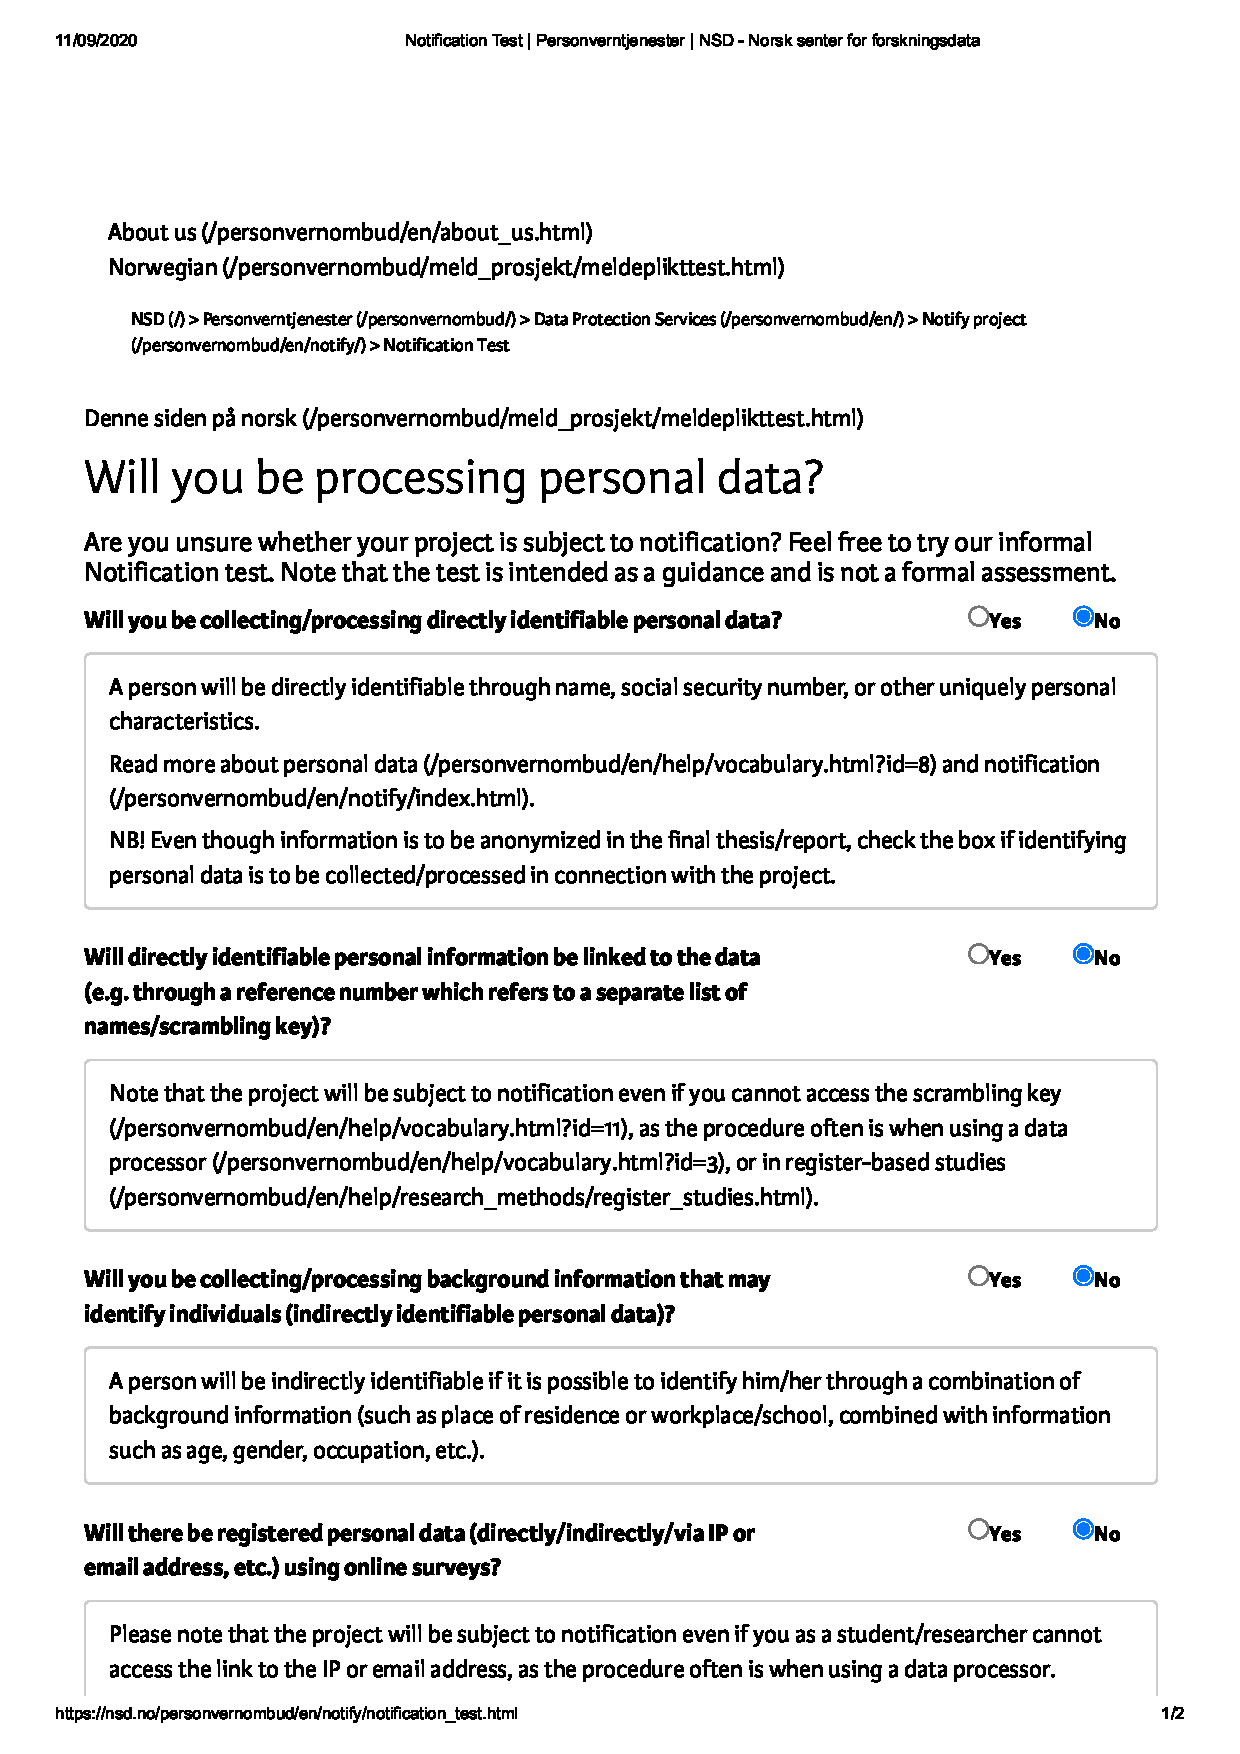
\includepdf[pages=-,fitpaper=true,noautoscale=true]{Appendices/Notification-Test.pdf}

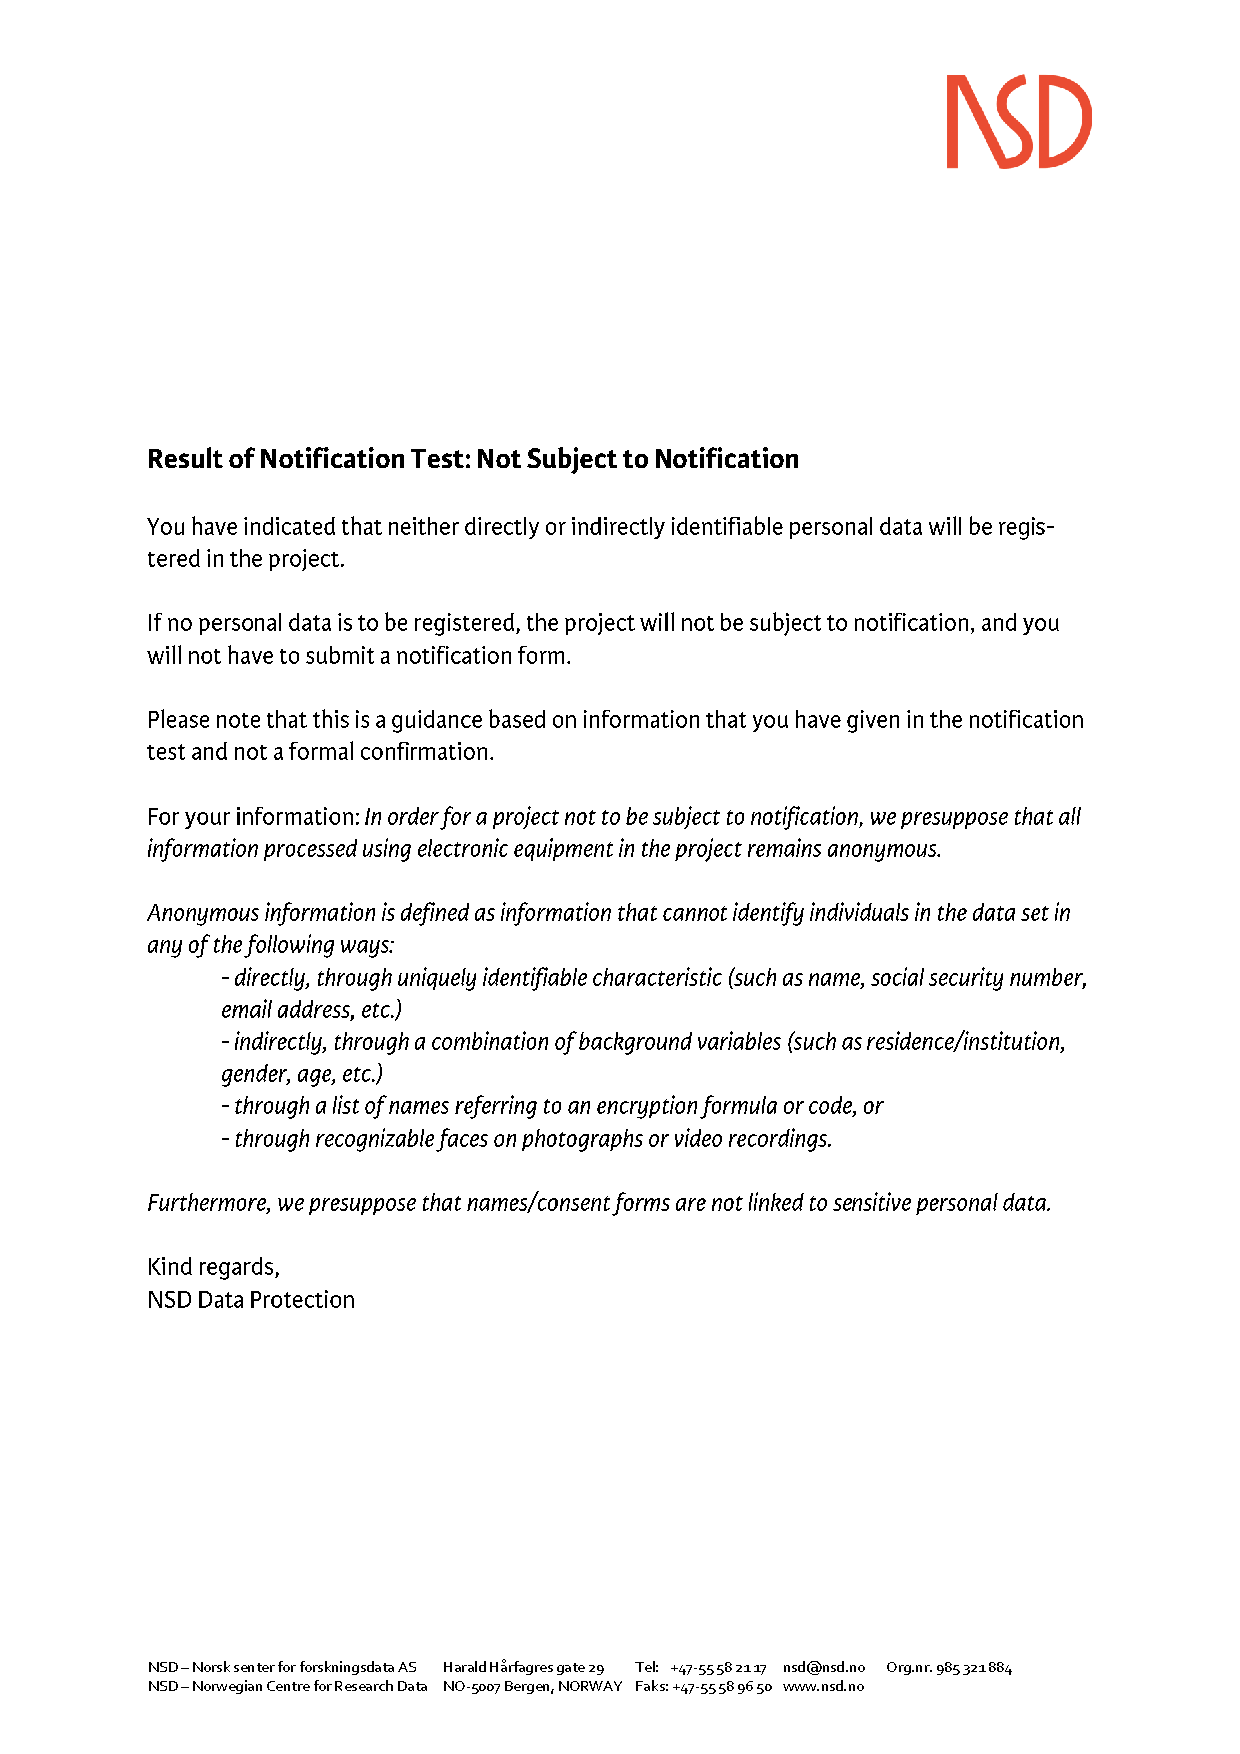
\includepdf[pages=-,fitpaper=true,noautoscale=true]{Appendices/not_subject_to_notification.pdf}


    \begin{singlespace}
    %\setcounter{secnumdepth}{0}
\chapter{Analysis Code}

\section{Chapter 1}

There is no analysis code in \cref{chp:1}.

\section{Chapter 2}

\subsection{Data Import} \label{R.import}
\begin{singlespace}\small
    \lstinputlisting[language=R,style=vscodeR]{./R/0 Import.R}
\end{singlespace}

\subsection{Missing Pattern Inspection} \label{R.missing}
\begin{singlespace}\small
    \lstinputlisting[language=R,style=vscodeR]{./R/1 Missing.R}
\end{singlespace}

\subsection{Data Reimport} \label{R.reimport}
\begin{singlespace}\small
    \lstinputlisting[language=R,style=vscodeR]{./R/2 Reimport.R}
\end{singlespace}

\subsection{Financial Knowledge Index} \label{R.fki}
\begin{singlespace}\small
    \lstinputlisting[language=R,style=vscodeR]{./R/4 FKI.R}
\end{singlespace}

    \end{singlespace}
    \chapter{Derivation of Country-level Financial Knowledge Indices}

%\epigraph{There are two things you are better off not watching in the making: sausages and\\ econometric estimates.}{Edward Leamer}

\section{Theoretical Foundation}

PISA 2018 financial literacy dataset \parencite{FLdata} provides rich information about students and schools. For the purpose of cross-country comparison, however, the country-level data must be addressed separately by the researchers. \textcite{morenoherrero:2018a}, for instance, introduced a variable ``quality of math and science education'' to control for country-level differences since consensus is yet to emerge about the most appropriate measure for ``countries' financial knowledge''. Inspired by the UN's approach to forming Human Development Indices, a recent publication \textcite{olivermarquez:2020} highlighted four aspects of countries' macroeconomic practices in their attempt to develop country-level financial knowledge indices (FKI).

Oliver-M{\'a}rquez and colleagues consider a country's economic capability, represented by its GDP per capita, to be a key dimension in bringing about its FKI. Secondly, literature converges on the importance of education training for a country's financial knowledge capability \parencite{oecd:2005}. Thirdly, countries with regular engagement with sophisticated financial products and financial markets should possess higher FKI. Lastly, countries with higher aggregate consumption levels and with ageing populations are likely to possess higher FKI due to more frequent exposure and pressure in retirement provision, respetively.

More specifically, \textcite{olivermarquez:2020} suggests using the logarithm of GDP per capital in current international dollars (purchasing power parity adjusted) as a measure for the \texttt{Economic Capability} sub-index. For the \texttt{Education Training} sub-index, the authors consider postgraduate-to-total-tertiary-graduation ratios as a reflection of ``highly skilled'' workforce and the mean years of schooling as a measure of countries' general education levels. For the \texttt{Use} sub-index, gross portfolio equity assets (GPEA) and insurance company assets (ICA) are considered sophisticated financial products countries engage themselves in. Additionally, in order to capture the central role of technology in amplifying the proliferation and use of financial assets, the proportion of Internet users (\textsc{IUS}) enters the definition via
\[ \texttt{Use} = ( \text{GPEA} + \text{ICA} ) ^ \text{IUS}. \]
For the final sub-index \texttt{Need}, the authors define
\[ \texttt{Need} = ( \text{PFA} + \text{AC} ) ^ \text{AGEING}, \]
where \textsc{PFA} is the pension-fund-assets-to-\textsc{GDP} ratio. Aggregate consumption is defined as:
\[ \text{AC} = \frac{2\% \times \text{household final consumption expenditure}}{\text{GDP}}, \]
where the ``$2\%$ rule'' is drawn from \textcite{caliendo:2013} and the proportion of ageing population is computed as
\[ \text{AGEING} = \frac{ \left[ \frac{\text{population}(>65)}{\text{population}(20 \sim 64)} \right]_{2018} - \left[ \frac{\text{population}(>65)}{\text{population}(20 \sim 64)} \right]_{2009} }{ \left[ \frac{\text{population}(>65)}{\text{population}(20 \sim 64)} \right]_{2009} }. \]

\section{Data Collection and Missing Data Treatment}

The data sources for FKI computation are documented in \cref{tab:FKIsource} and its associated notes. The sub-indices \texttt{Educational Training} and \texttt{Use} both contain missing observations for the year 2018. Majority of such missing data appear to be the result of administrative delay, with historic observations available until 2017. It is therefore feasible to conduct time-series forecasts using prior year observations to best approximate 2018 values.

\ltable{tab:FKIsource}{Data Sources for FKI Computation}{
    \begin{tabular}{cclc}
    \toprule
    \multicolumn{1}{c}{Database$\ ^\text{a}$} & Country$\ ^\text{b}$ & \multicolumn{1}{c}{Series} & Time \\
    \midrule
    \rowcolor[rgb]{ .9,  .9,  .9} \multicolumn{4}{c}{Economic Capacity} \\
    WB-dev & 20    & GDP per capita, PPP (current international \$) & 2018 \\
    \rowcolor[rgb]{ .9,  .9,  .9} \multicolumn{4}{c}{Educational Training} \\
    WB-ed & 20 \textbackslash\ Russia & Graduates from ISCED 7 programmes in tertiary education, both sexes (number) & 2013--\textbf{2018} \\
          &       & Graduates from ISCED 8 programmes in tertiary education, both sexes (number) & 2013--\textbf{2018} \\
          &       & Graduates from tertiary education, both sexes (number) & 2013--\textbf{2018} \\
    RS & Russia & PhD (Type 1)$\ ^\text{c}$, PhD (Type 2)$\ ^\text{d}$ & 2018 \\
    RE & Russia & Master (Type 1)$\ ^\text{e}$, Master (Type 2)$\ ^\text{f}$, total tertiary \emph{excluding} PhD$\ ^\text{g}$ & 2018 \\
    HDR & 20    & Dimension = Education; Education = Mean years of schooling (years) & 2018 \\
    \rowcolor[rgb]{ .9,  .9,  .9} \multicolumn{4}{c}{Use} \\
    WB-fin & 20    & Gross portfolio equity assets to GDP (\%) & 2011--\textbf{2018} \\
           &       & Insurance company assets to GDP (\%) & 2011--\textbf{2018} \\
    WB-dev & 20    & Individuals using the Internet (\% of population) & 2009--\textbf{2018} \\
    \rowcolor[rgb]{ .9,  .9,  .9} \multicolumn{4}{c}{Need} \\
    WB-fin & 20 \textbackslash\ Georgia & Pension fund assets to GDP (\%) & 2008--\textbf{2018} \\
    GP & Georgia & Minutes of the meeting of the investment board of the Pension Agency$\ ^\text{h}$ & $\textcolor{white}{\ ^\text{*}}$2019$\ ^\text{*}$ \\
    GS & Georgia & GDP at current prices, billion GEL$\ ^\text{i}$ & 2018 \\
    WB-dev & 20    & Household and NPISHs final consumption expenditure, PPP (current international \$) & 2018 \\
          &       & GDP, PPP (current international \$) & 2018 \\
          &       & Population ages 0--14, male & 2009, 2018 \\
          &       & Population ages 0--14, female & 2009, 2018 \\
          &       & Population ages 15--64, male & 2009, 2018 \\
          &       & Population ages 15--64, female & 2009, 2018 \\
          &       & Population ages 65 and above, male & 2009, 2018 \\
          &       & Population ages 65 and above, female & 2009, 2018 \\
          &       & Population ages 15--19, male (\% of male population) & 2009, 2018 \\
          &       & Population ages 15--19, female (\% of female population) & 2009, 2018 \\
          \bottomrule
    \end{tabular}
}{Sub-indices are shaded in gray. Bold font signifies this year contains missing data.}{3}
\newpage

\begin{singlespace} \small
\begin{itemize}
    \item[$^\text{a}$] WB-dev = \href{https://databank.worldbank.org/source/world-development-indicators}{World Bank -- World development indicators}\\
        WB-ed = \href{https://databank.worldbank.org/source/education-statistics-^-all-indicators}{World Bank -- Education statistics -- All indicators}\\
        WB-fin = \href{https://databank.worldbank.org/source/global-financial-development}{World Bank -- Global financial development}\\
        HDR = \href{http://hdr.undp.org/en/data}{Human Development Reports -- Data}\\
        RS = \href{https://rosstat.gov.ru/}{Russian Federal State Statistic Service}\\
        RE = \href{https://minobrnauki.gov.ru}{Russian Ministry of Education and Science}\\
        GP = \href{https://www.pensions.ge}{Pension Agency of Georgia}\\
        GS = \href{https://www.geostat.ge}{National Statistics Office of Georgia}
    \item[$^\text{b}$] ``20'' = the 20 participating countries in 2018 \textsc{PISA} financial literacy test: Brazil, Bulgaria, Canada, Chile, Estonia, Finland, Georgia, Indonesia, Italy, Latvia, Lithuania, the Netherlands, Peru, Poland, Portugal, Russian Federation, Serbia, Slovak Republic, Spain, and the USA. ``\textbackslash'' = exluding or except
    \item[$^\text{c}$] \href{https://rosstat.gov.ru/storage/mediabank/asp-2(1).xls}{https://rosstat.gov.ru/storage/mediabank/asp-2(1).xls}, Sheet ``\foreignlanguage{russian}{по направлениям подготовки}'', Cell C7 = number of PhD graduates \mbox{(Type 1)}
    \item[$^\text{d}$] \href{https://rosstat.gov.ru/storage/mediabank/asp-3.xls}{https://rosstat.gov.ru/storage/mediabank/asp-3.xls}, Sheet ``\foreignlanguage{russian}{по научным специальностям}'', Cell B7 = number of PhD graduates \mbox{(Type 2)}
    \item[$^\text{e--g}$] \href{https://minobrnauki.gov.ru/common/upload/download/VPO_1_2018.rar}{https://minobrnauki.gov.ru/common/upload/download/VPO{\textunderscore}1{\textunderscore}2018.rar} contains a spreadsheet \textcolor{blue}{\foreignlanguage{russian}{СВОД{\textunderscore}ВПО1{\textunderscore}ВСЕГО}.xls}, Sheet ``P2{\textunderscore}1{\textunderscore}3(1)'', Cell E198 = number of master graduates (Type 1)$^\text{e}$, Cell E410 = number of master graduates (Type 2)$^\text{f}$, Cell E592 = total tertiary graduates \emph{excluding} PhD$^\text{g}$
    \item[$^\text{h}$] \href{https://www.pensions.ge/docs/legislation/investment-board-protocol-4.pdf}{Minutes of the meeting of the investment board of the Pension Agency}, p. 4, no. 3
    \item[$^\text{i}$] \href{https://www.geostat.ge/en/modules/categories/23/gross-domestic-product-gdp}{Gross domestic product (GDP)}, row = GDP at current prices, billion GEL, column = 2018
    \item[$^\text{*}$] Georgia started a \href{https://agenda.ge/en/news/2019/13}{new pension system} on 1 January 2019. Since 2018 was a transitional period with scarce data, 2019 is used as the best approximation for Georgia's pension system for 2018.
\end{itemize}
\end{singlespace}

\clearpage



\subsection{Sub-index \texttt{Educational Training}}

The 2018 archive for the number of master (ISCED 7), PhD (ISCED 8), and total tertiary graduates are incomplete for all participating countries except Georgia, Indonesia and Serbia. \cref{fig:skilled} presents a time series plot of
\[ \texttt{highly skilled} = \frac{\text{number of masters} + \text{number of PhDs}}{\text{total number of tertiary graduates}} \]
and suggests that this ratio is likely to be stable over time, especially between adjacent years. A ``naive forecast'', where the nearest available year's data are to be duplicated for 2018, is applied for \texttt{highly skilled}.

\pfigure{fig:skilled}{Proportion of Postgraduates to Total Tertiary Graduations}{1}{./Figures/skilled.pdf}{``Postgraduate'' is defined as master (ISCED 7) and PhD (ISCED 8) graduates. Countries not shown: GEO, IDN and SRB (2018 data available) and RUS (consult other sources)}{1.75}{1.25}

\subsection{Sub-index \texttt{Use}}

All series involved in calculating this sub-index, GPEA, ICA and IUS, contain missing data. When time series data contain only exponential growth but no underlying trend, a simple exponential smoothing would suffice \parencite{garder:1985}; if trend is present, Holt-Winters method is superior \parencite{chatfield:1978}. \cref{fig:use} facilitates this decision making by plotting both the original and log-transformed versions of GPEA and ICA series. Since curves after log-transformations have slopes, it is prudent to apply the Holt-Winters forecasting method in order to account for possible trends contained in the original series.

\pfigure{fig:use}{Time Series Trend Test}{1}{./Figures/use.pdf}{The time series plots after natural logarithm transformations (bottom panels) are not flat, suggesting the original series (top panels) contain trends. Holt-Winters method therefore is preferred over simple exponential smoothing for 2018 forecasts.}{0.5}{0.85}

The IUS series contains missing data for Canada, Chile and the United States. Similar Holt-Winters procedure is applied to recover 2018 IUS data.

\ltable{tab:FKIraw}{Data Utilised for Computing FKI}{
  \begin{tabular}{cd{3} c d{3}d{1} c d{3}d{3}d{3} c d{3}d{3}d{3}}
    \toprule
    & \multicolumn{1}{c}{Economic Capacity} &       & \multicolumn{2}{c}{Educational Training} &       & \multicolumn{3}{c}{Use} &       & \multicolumn{3}{c}{Need} \\
\cmidrule{2-2}\cmidrule{4-5}\cmidrule{7-9}\cmidrule{11-13}          & \multicolumn{1}{c}{GDP per capita} &       & \multicolumn{1}{c}{Skilled} & \multicolumn{1}{c}{Schooling} &       & \multicolumn{1}{c}{GPEA} & \multicolumn{1}{c}{ICA} & \multicolumn{1}{c}{IUS} &       & \multicolumn{1}{c}{PFA} & \multicolumn{1}{c}{AC} & \multicolumn{1}{c}{AGEING} \\
    \midrule
    BRA   & 9.612 &       & 6.484 & 7.8   &       & 1.683 & 16.259 & 70.434 &       & 11.827 & 1.21  & 0.288 \\
    BGR   & 10.026 &       & 45.294 & 11.8  &       & 4.114 & 7.044 & 64.782 &       & 13.577 & 1.091 & 0.234 \\
    CHL   & 10.117 &       & 16.371 & 10.4  &       & 51.755 & 25.591 & 89.531 &       & 73.225 & 1.073 & 0.214 \\
    EST   & 10.501 &       & 36.765 & 13    &       & 16.399 & 7.681 & 89.357 &       & 18.012 & 0.876 & 0.163 \\
    FIN   & 10.807 &       & 35.024 & 12.4  &       & 93.626 & 31.481 & 88.89 &       & 52.024 & 0.974 & 0.37 \\
    GEO   & 9.588 &       & 24.039 & 12.8  &       & 0.784 & 1.469 & 62.718 &       & 0.834 & 1.227 & 0.042 \\
    IDN   & 9.362 &       & 7.771 & 8     &       & 0.636 & 4.612 & 39.905 &       & 1.826 & 1.059 & 0.145 \\
    ITA   & 10.665 &       & 44.771 & 10.2  &       & 57.434 & 51.26 & 74.387 &       & 10.589 & 1.075 & 0.155 \\
    LVA   & 10.33 &       & 29.554 & 12.8  &       & 8.598 & 2.538 & 83.577 &       & 14.732 & 1.027 & 0.142 \\
    LTU   & 10.487 &       & 28.749 & 13    &       & 9.008 & 5.5   & 79.723 &       & 7.457 & 1.107 & 0.149 \\
    NLD   & 10.961 &       & 32.59 & 12.2  &       & 124.171 & 64.956 & 94.712 &       & 207.938 & 0.805 & 0.326 \\
    PER   & 9.479 &       & 13.577 & 9.2   &       & 16.027 & 6.505 & 52.54 &       & 22.53 & 1.187 & 0.227 \\
    POL   & 10.368 &       & 36.725 & 12.3  &       & 4.853 & 9.535 & 77.542 &       & 9.838 & 1.085 & 0.355 \\
    PRT   & 10.444 &       & 34.454 & 9.2   &       & 19.353 & 25.579 & 74.661 &       & 8.761 & 1.133 & 0.237 \\
    RUS   & 10.267 &       & 30.349 & 12    &       & 0.302 & 2.614 & 80.865 &       & 4.415 & 0.941 & 0.155 \\
    SRB   & 9.774 &       & 26.946 & 11.2  &       & 0.306 & 5.111 & 73.361 &       & 0.845 & 1.171 & 0.28 \\
    SVK   & 10.391 &       & 54.417 & 12.6  &       & 10.644 & 8.873 & 80.66 &       & 12.497 & 0.962 & 0.3 \\
    ESP   & 10.609 &       & 33.929 & 9.8   &       & 27.681 & 28.23 & 86.107 &       & 10.235 & 1.044 & 0.186 \\
    USA   & 11.048 &       & 24.825 & 13.4  &       & 55.505 & 30.183 & 84.881 &       & 150.04 & 1.364 & 0.252 \\
    \bottomrule
    \end{tabular}
}{Full variable names: Skilled = Postgraduate to total tertiary ratio; Schooling = Mean year of schooling; GPEA = Gross portfolio to GDP ratio; ICA = Insurance company assets to GDP ratio; IUS = Number of Internet users per 100 population; PFA = Pension fund assets to GDP ratio; AC = 2\% of household final consumption expenditure to GDP ratio; AGEING = Aged-to-productive-population ratio (\% change between 2009 and 2018)}{3}


\subsection{Other Items with Data Concerns}

Russia reported 67.96\% and 61.01\% of its total university degree receipients to be postgraduates for the year 2013 and 2015 respectively (2014 missing). This figure rapidly declines to 41.6\% in 2016 and further down to 25.69\% in 2017. Such volatility goes against the stable patterns shared by most countries in \cref{fig:skilled}, casting doubt on data reliability. Separate investigation is therefore conducted using Russian government archive (Notes c to g in \cref{tab:FKIsource}).

Georgia underwent pension reform in 2018 with fund balance gradually transitioning to State Pension Agency for its official resumption of duty on 1 January 2019. Resultantly, 2018 pension balance for this country is unavailable but to be best appoximated using 2019 official data (Notes h, i and * of \cref{tab:FKIsource}).

\cref{tab:FKIraw} documents the results of the abovementioned data recovery process.

\section{Standardisation, Weights and FKI}

Following \textcite{olivermarquez:2020}'s procedure, all series in \cref{tab:FKIraw} undergo min-max normalisation such that the smallest entry receives a new score of $0.01$ and the biggest number is re-coded to $0.99$. This slight deviation from the original paper (where the min-max normalisation yields $0$ to $1$) is to avoid multiplying a series by zero or raising a base to the power of zero.

Variable weights are calculated following \textcite{olivermarquez:2020}'s recipe to be the inverses of each series' standard deviations. Whereas a sub-index combines more than one series, each weight is further divided by the sum of the constituent weights so that total weights add to one.

FKI is finally computed by taking the geometric mean of all four sub-indices, subject to sub-index-weights similar to variable weights above, as presented in \cref{tab:FKI}.

\ptable{tab:FKI}{FKI and Sub-indices}{
    \begin{tabular}{c c d{3} c d{3}d{3}d{3}d{3}}
\toprule
        && \multicolumn{1}{c}{FKI}       && \multicolumn{1}{c}{EC}        & \multicolumn{1}{c}{ET}        & \multicolumn{1}{c}{Use}       & \multicolumn{1}{c}{Need}\\
\midrule
        USA   &       & 1.029 &       & 0.990 & 0.590 & 1.467 & 1.580 \\
        ITA   &       & 0.810 &       & 0.767 & 0.601 & 1.603 & 0.767 \\
        ESP   &       & 0.661 &       & 0.734 & 0.464 & 1.012 & 0.670 \\
        LTU   &       & 0.609 &       & 0.664 & 0.633 & 0.325 & 0.801 \\
        PRT   &       & 0.606 &       & 0.639 & 0.401 & 0.869 & 0.719 \\
        CHL   &       & 0.589 &       & 0.449 & 0.302 & 1.372 & 0.939 \\
        EST   &       & 0.576 &       & 0.672 & 0.747 & 0.419 & 0.455 \\
        SVK   &       & 0.552 &       & 0.608 & 0.924 & 0.414 & 0.341 \\
        POL   &       & 0.546 &       & 0.595 & 0.700 & 0.354 & 0.503 \\
        GEO   &       & 0.369 &       & 0.141 & 0.548 & 0.174 & 0.997 \\
        PER   &       & 0.289 &       & 0.078 & 0.194 & 0.780 & 0.868 \\
        BRA   &       & 0.131 &       & 0.155 & 0.010 & 0.506 & 0.809 \\
        IDN   &       & 0.104 &       & 0.010 & 0.040 & 0.975 & 0.734 \\
\bottomrule
    \end{tabular}
}{Table sorted in descending order by countries' FKI. FKI = financial knowledge index, EC = Economic Capability, ET = Educational Training.}{2.5}


%    \chapter{Multilevel Multiple Imputation}
\label{app:MMI}

\section{\textsf{Mplus} Input Code}
\label{sec:MMI_inp}

\lstinputlisting[style=vscodeMplus]{./Mplus/MMI/MMI.inp}

\section{Selected \textsf{Mplus} Output}
\label{sec:MMI_out}

\lstinputlisting[style=vscodeMplus_out,linerange={2909-2967}]{./Mplus/MMI/MMI.out}

\section{Diagnostic Plots}
\label{sec:MMI_diagnostic}

\newpage

% Table generated by Excel2LaTeX from sheet 'Sheet1'
\ltable{tab:MMI}{Summary of Diagnostic Plots of Multilevel Multiple Imputation}{
      \begin{tabular}{ccclrrccc}
\toprule
      Parameter & \multicolumn{1}{c}{Parameter} & Modelling & \multicolumn{1}{c}{Brief} & \multicolumn{1}{c}{Posterior} & \multicolumn{1}{c}{Posterior} & 95\% credibility & Chain & AR-free \\
      number & \multicolumn{1}{c}{label} & level & \multicolumn{1}{c}{description} & \multicolumn{1}{c}{mean} & \multicolumn{1}{c}{variance} & interval & converged & chains \\
\midrule
      1     & \texttt{MALE}  & Within & Whether participant is male & 0.502 &       & (0.499, 0.505) & Yes   & 4 \\
      2     & \texttt{IMMI1GEN} & Within & Whether participant migrated to this country & 0.029 &       & (0.028, 0.030) & Yes   & 4 \\
      3     & \texttt{IMMI2GEN} & Within & Whether their parent did & 0.042 &       & (0.041, 0.044) & Yes   & 4 \\
      4     & \texttt{ESCS}  & Within & Index of economic, social and cultural status & $-$0.241 &       & ($-$0.247, $-$0.234) & Yes   & 4 \\
      5     & \texttt{FCFMLRTY} & Within & Familiarity with concepts of finance & 7.049 &       & (7.015, 7.083) & Yes   & 4 \\
      6     & \texttt{FLCONFIN} & Within & Confidence about financial matters & $-$0.072 &       & ($-$0.079, $-$0.065) & Yes   & 4 \\
      7     & \texttt{FLSCHOOL} & Within & Financial education in school lessons & 0.018 &       & (0.011, 0.024) & Yes   & 4 \\
      8     & \texttt{NOBULLY} & Within & Participant's experience of being bullied (reverse) & $-$0.059 &       & ($-$0.067, $-$0.052) & Yes   & 4 \\
      9     & \texttt{FLFAMILY} & Within & Parental involvement in matters of financial literacy & 0.064 &       & (0.057, 0.070) & Yes   & 4 \\
            &       &       &       &       &       &       &       &  \\
      10    & \texttt{MALE}  & Within & Whether participant is male &       & 0.250 & (0.248, 0.252) & Yes   & 4 \\
      11    & \texttt{IMMI1GEN} & Within & Whether participant migrated to this country &       & 0.028 & (0.028, 0.028) & Yes   & 4 \\
      12    & \texttt{IMMI2GEN} & Within & Whether their parent &       & 0.041 & (0.040, 0.041) & Yes   & 4 \\
      13    & \texttt{ESCS}  & Within & Index of economic, social and cultural status &       & 1.183 & (1.173, 1.193) & Yes   & 4 \\
      14    & \texttt{FCFMLRTY} & Within & Familiarity with concepts of finance &       & 29.754 & (29.495, 30.016) & Yes   & 4 \\
      15    & \texttt{FLCONFIN} & Within & Confidence about financial matters &       & 1.034 & (1.025, 1.044) & Yes   & 4 \\
      16    & \texttt{FLSCHOOL} & Within & Financial education in school lessons &       & 1.040 & (1.031, 1.049) & Yes   & 4 \\
      17    & \texttt{NOBULLY} & Within & Participant's experience of being bullied (reverse) &       & 1.111 & (1.100, 1.121) & Yes   & 4 \\
      18    & \texttt{FLFAMILY} & Within & Parental involvement in matters of financial literacy &       & 1.090 & (1.080, 1.100) & Yes   & 4 \\
            &       &       &       &       &       &       &       &  \\
      19    & \texttt{STRAIO} & Between & Student$-$teacher ratio & 13.873 &       & (13.607, 14.139) & Yes   & 4 \\
      20    & \texttt{EDUSHORT} & Between & Shortage of educational material & 0.131 &       & (0.106, 0.157) & Yes   & 4 \\
            &       &       &       &       &       &       &       &  \\
      21    & \texttt{STRAIO} & Between & Student$-$teacher ratio &       & 103.532 & (99.750, 107.430) & Yes   & 4 \\
      22    & \texttt{EDUSHORT} & Between & Shortage of educational material &       & 1.074 & (1.037, 1.112) & Yes   & 4 \\
\bottomrule
      \end{tabular}
}{Notes go here.}{6}
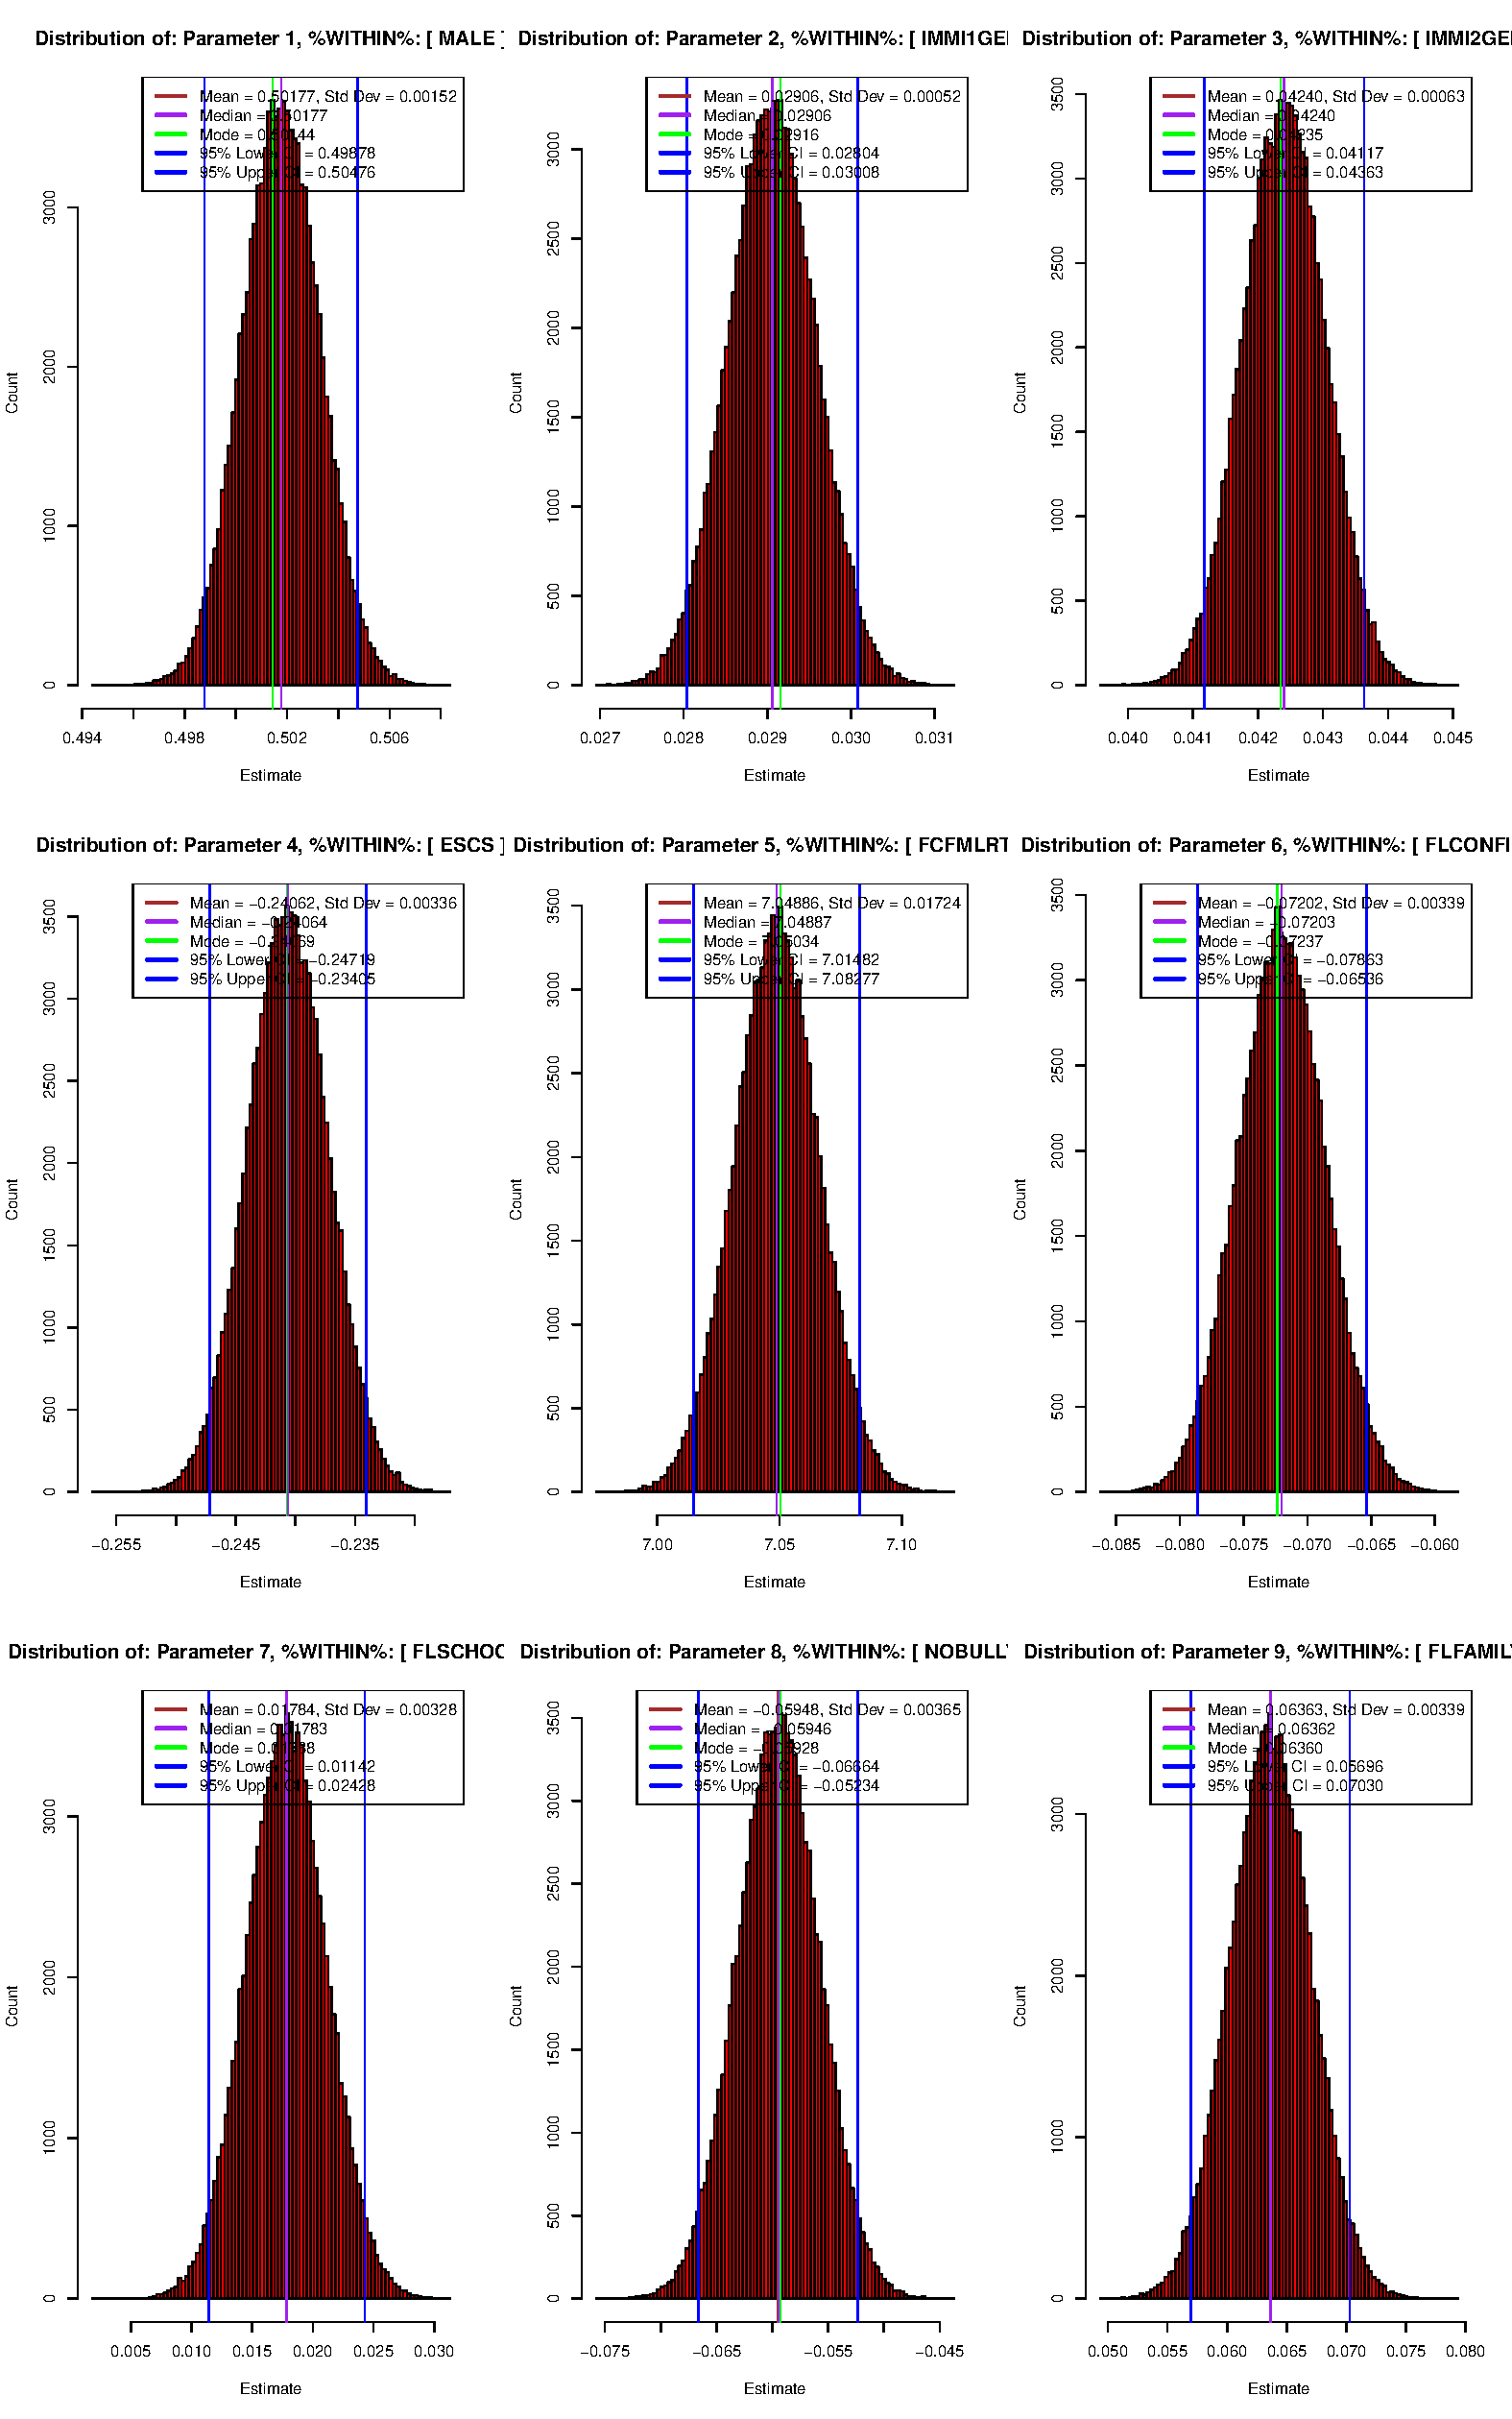
\includepdf[pages=-,width=\textwidth]{./Figures/MMI_diagnostic.pdf}

%    \include{Appendices/E}
%    \include{Appendices/F}
     \chapter{Review of Matrix Calculus}

\section{Notations}

Let us first establish the notation. This is important because bad notation is a serious obstacle to elegant mathematics and coherent exposition and it can be misleading.

Unless specified otherwise, $\phi$ denotes a scalar function; $\m{f}$ a vector function and $\m{F}$ a matrix function. Also, $x$ denotes a scalar argument, $\m{x}$ a vector argument and $\m{X}$ a matrix argument. For example, we write

\begin{table*}[h]
  \begin{center}
  \begin{tabular}{lll}
    $\phi(x)=x^2$     &$\phi(\m{x})=\T{a}\m{x}$       &$\phi(\m{X})=\tr{\T{X}\m{X}}$\\
    $\m{f}(x)=
      \begin{pmatrix}
        x\\
        x^2
      \end{pmatrix}$    &$\m{f}(\m{x})=\m{Ax}$    &$\m{f}(\m{X})=\m{Xa}$\\
      $\m{F}(x)=x^2\Id{m}$  &$\m{F}(\m{x})=\m{x}\T{x}$  &$\m{F}(\m{X})=\T{X}$
  \end{tabular}
\end{center}
\end{table*}

Since the prime notation $'$ may easily cause confusion between derivatives and transposes, preference is given to the Leibniz notation $\frac{\dd}{\dd x}$ for derivatives and $\T{}$ for transposes---unless this system becomes too cumbersome, in which case $\m{f}'(\m{x})$ will denote derivatives and $\m{f}(\m{x})'$ for transposes.

\section{Derivatives and differentials}

\subsection{Derivative}

\theoremstyle{definition}
\begin{definition}[Derivatives]\label{Def.D}
  If $\m{f}$ is an $m\times 1$ vector function of an $n\times 1$ vector $\m{x}$, then the \emph{derivative} (or \emph{Jacobian matrix}) of $\m{f}$ is the $m\times n$ matrix
  \begin{equation}\label{Eq.Def.D}
    \D\m{f}(\m{x}):=\frac{\partial\m{f}(\m{x})}{\partial\T{x}},
  \end{equation}
  whose elements are the partial derivatives
  \begin{equation*}
    \frac{\partial f_i(\m{x})}{\partial x_j},\ \text{for}\ %
    \begin{aligned}
      i&=1,\cdots,m,\\
      j&=1,\cdots,n.
    \end{aligned}
  \end{equation*}
\end{definition}

\subsection{Differential}

In the one dimensional case, the equation
\begin{equation}\label{Eq.D}
  \lim_{u\to 0}\frac{\phi(x+u)-\phi(x)}{u}=\phi'(x)
\end{equation}
defines the derivative of $\phi$ at $x$. Rewriting \cref{Eq.D} gives
\begin{equation}\label{Eq.d}
  \phi(x+u)=\phi(x)+\phi'(x)u+O(u),
\end{equation}
where the remainder term $O(u)$ quickly vanishes as $u$ approaches $0$.

\theoremstyle{definition}
\begin{definition}[Differential]
  We define the (first) \emph{differential} of $\phi$ at $x$ (with increment $u$) as
  \begin{equation}
    \dd\phi(x;u)=\phi'(x)u.
  \end{equation}
\end{definition}

For example, for $\phi(x)=x^2$, we have $\dd\phi(x;u)=2xu$. In practice, we write $\dd x$ instead of $u$, so that $\dd\phi(x)=\phi'(x)\dd x=2x\dd x.$

In the vector case, similar to \cref{Eq.d}, we have
\begin{equation}
  \m{f}(\m{x}+\m{u})=\m{f}(\m{x})+[\D\m{f}(x)]\m{u}+O(\m{u}),
\end{equation}
and the (first) differential is defined as
\begin{equation}
  \dd\m{f}(\m{x};\m{u})=[\D\m{f}(x)]\m{u}.
\end{equation}

Although rarely used in econometrics, for completeness, the matrix case can be obtained from the vector case by writing $\m{f}:=\vec{F}$ and $\m{x}:=\vec{X}$.

\subsection{Which to use?}

For practical rather than theoretical reasons, the treatment of matrix calculus is based on differentials ($\dd\m{f}$) rather than derivatives ($\D\m{f}$) because the former yields a result with the same dimension as $\m{f}$. For example, consider $\md{f}{m}{1}(\md{x}{n}{1})$ (reading ``$\m{f}$ being an $m\times 1$ vector function of an $n\times 1$ vector $\m{x}$''), $\D\m{f}(\m{x})$ is an $m\times n$ matrix (due to \cref{Def.D}) whereas $\dd\m{f}(\m{x})$ remains an $m\times 1$ vector (same as $\m{f}$). The advantage is even larger for matrices: for $\md{F}{m}{p}(\md{X}{n}{q})$, $\dd\m{F}(\m{X})$ has the same dimension as $\m{F}$ irrespective of the dimension of $\m{X}$, but $\D\m{F}(\m{X})$ is going to be a horrendous $mp\times nq$ matrix.

\section{Layout convention}\label{S.layout}

Under the \emph{numerator layout}, when we differentiate a scalar function $\phi$ \wrt a column vector $\md{x}{n}{1}$, we get a \emph{row} vector of dimension $1\times n$. If we want our result to be in the column form, we must differentiate $\phi$ \wrt a row vector to start with. This is why the denominator in \cref{Eq.Def.D} contains a transpose.

\section{Application in OLS}

\subsection{Background}

Imagine we are interested in learning the return on education. We might propose a rather simple model
\begin{equation}
  \texttt{inc}=\beta_0+\beta_1\texttt{edu}+\beta_2\texttt{exp}+\epsilon
\end{equation}
where \texttt{inc} is one's income, \texttt{edu} and \texttt{exp} denote years of formal education and years spent in the labour market, respectively.

We managed to collect survey data from $n$ respondents and organised this information in the following system of equations:
\begin{equation}
  \left\{
    \begin{aligned}
      \texttt{inc}_1 &= \beta_0+\beta_1\texttt{edu}_1+\beta_2\texttt{exp}_1+\epsilon_1\\
      \texttt{inc}_2 &= \beta_0+\beta_1\texttt{edu}_2+\beta_2\texttt{exp}_2+\epsilon_2\\
      \cdots\\
      \texttt{inc}_n &= \beta_0+\beta_1\texttt{edu}_n+\beta_2\texttt{exp}_n+\epsilon_n\\
    \end{aligned}
  \right.
\end{equation}

This system of linear equations can be represented in the matrix notation using
\begin{equation}
  \md{y}{n}{1}=
    \begin{pmatrix}
      \texttt{inc}_1\\
      \texttt{inc}_2\\
      \cdots\\
      \texttt{inc}_2\\
    \end{pmatrix},\ %
  \md{X}{n}{3}=
    \begin{pmatrix}
      1     &\texttt{edu}_1     &\texttt{exp}_1\\
      1     &\texttt{edu}_2     &\texttt{exp}_2\\
      \cdots\\
      1     &\texttt{edu}_n     &\texttt{exp}_n\\
    \end{pmatrix},\ %
  \md{\beta}{3}{1}=
    \begin{pmatrix}
      \beta_0\\
      \beta_1\\
      \beta_2\\
    \end{pmatrix},\ \text{and}\ %
  \md{\epsilon}{n}{1}=
    \begin{pmatrix}
      \epsilon_1\\
      \epsilon_2\\
      \cdots\\
      \epsilon_n\\
    \end{pmatrix}
  \end{equation}
as
\begin{equation}\label{Eq.setup}
  \m{y}=\m{X\beta}+\m{\epsilon}.
\end{equation}

\subsection{Ordinary least squares}

The objective of OLS is to minimise the \emph{sum of squared} error terms. A handy way of representing sum of squared $\epsilon$ is
\begin{equation}
  \text{SSE}=\sum_{i=1}^n\epsilon_i^2=\epsilon_1^2+\epsilon_2^2+\cdots+\epsilon_n^2=
  \begin{pmatrix}
    \epsilon_1      &\epsilon_2     &\cdots      &\epsilon_n
  \end{pmatrix}
  \begin{pmatrix}
    \epsilon_1\\
    \epsilon_2\\
    \cdots\\
    \epsilon_n
  \end{pmatrix}
  =\T{\epsilon}\m{\epsilon}.
\end{equation}
In fact, $\T{x}\m{x}$ is the mathematical translation of ``sum of squared'' of $\m{x}$.

Now we are ready to continue. We want to carefully choose a combination of $\beta_0$, $\beta_1$ and $\beta_2$ in order to make SSE as small as possible, ie
\begin{equation}\label{Eq.min}
  \min{\T{\epsilon}\m{\epsilon}}{\m{\beta}}=\min{\left(\m{y}-\m{X\beta}\right)\Ts\left(\m{y}-\m{X\beta}\right)}{\m{\beta}}
\end{equation}
(the equal sign is due to \cref{Eq.setup}).

Two observations can be made from the minimisation problem in \cref{Eq.min}:
\begin{enumerate}
  \item both $\m{y}$ and $\m{X}$ are collected data therefore can no longer be changed by the researcher; but we are free to adjust $\m{\beta}$ in whatever way we want, meaning $\m{\beta}$ is the ``independent variable'' and SSE is a function of $\m{\beta}$, and
  \item $\T{\epsilon}\m{\epsilon}$ is a scalar function (please verify).
\end{enumerate}
Then,
\begin{equation}
  \begin{aligned}
    \phi(\m{\beta})=\T{\epsilon}\m{\epsilon}&=\left(\m{y}-\m{X\beta}\right)\Ts\left(\m{y}-\m{X\beta}\right)\\
  &=\left(\T{y}-\T{\beta}\T{X}\right)\left(\m{y}-\m{X\beta}\right)\\
  &=\T{y}\m{y}-\T{y}\m{X\beta}-\T{\beta}\T{X}\m{y}+\T{\beta}\T{X}\m{X\beta}
  \end{aligned}
\end{equation}

We now differentiate $\phi(\m{\beta})$ \wrt $\m{\beta}$:
\begin{equation}\label{Eq.normal}
  \begin{aligned}
    \frac{\dd \phi(\m{\beta})}{\dd\m{\beta}}&=-\T{y}\m{X}-\frac{\dd}{\dd\m{\beta}}\left[\left(\T{\beta}\T{X}\m{y}\right)\Ts\right]+\T{\beta}\T{X}\m{X}+\frac{\dd}{\dd\m{\beta}}\left[\left(\T{\beta}\T{X}\m{X\beta}\right)\Ts\right]\\
    &=-\T{y}\m{X}-\frac{\dd}{\dd\m{\beta}}\left[\T{y}\m{X}\m{\beta}\right]+\T{\beta}\T{X}\m{X}+\frac{\dd}{\dd\m{\beta}}\left[\T{\beta}\T{X}\m{X}\m{\beta}\right]\\
    &=-\T{y}\m{X}-\T{y}\m{X}+\T{\beta}\T{X}\m{X}+\T{\beta}\T{X}\m{X}\\
    &=-2\T{y}\m{X}+2\T{\beta}\T{X}\m{X}
  \end{aligned}
\end{equation}
(We were able to liberally apply transpose to terms containing $\T{\beta}$ and not to others because $\phi$ is a scalar function and each term in it must also be $1\times 1$ in dimension, whose transpose must be equal to itself.)

Apply first order condition to \cref{Eq.normal}. An optimal $\hat{\beta}$ must satisfy
\begin{equation}\label{Eq.FOC}
  \begin{aligned}
    -2\T{y}\m{X}+2\hat{\beta}\Ts\T{X}\m{X}&=\Z\\
    2\hat{\beta}\Ts\T{X}\m{X}&=2\T{y}\m{X}\\
    \hat{\beta}\Ts\T{X}\m{X}&=\T{y}\m{X}\\
    \left(\hat{\beta}\Ts\T{X}\m{X}\right)\Ts&=\left(\T{y}\m{X}\right)\Ts\\
    \T{X}\m{X}\hat{\beta}&=\T{X}\m{y}\\
    \hat{\beta}&=\inv{\T{X}\m{X}}\T{X}\m{y}
  \end{aligned}
\end{equation}

Notice that another transpose was applied to Line 4 of \cref{Eq.FOC} in order to correct $\hat{\beta}\Ts$ (due to \cref{S.layout}) back to its column form $\hat{\beta}$. In fact, it would be better to do $\frac{\dd\phi(\m{\beta})}{\dd\T{\beta}}$ in \cref{Eq.normal} to avoid this later flipping. But the downside of this approach is a pedagogical one: most students would find differentiating \wrt $\T{\beta}$ out of blue while \wrt $\m{\beta}$ is much more natural. In further derivations, $\frac{\dd\phi(\m{\beta})}{\dd\T{\beta}}$ will be used.


\end{appendices}

% Put Index here
%\begin{multicols}{2}
\cleardoublepage
\phantomsection
\addcontentsline{toc}{chapter}{Name Index}
\printindex[a]

\cleardoublepage
\phantomsection
\addcontentsline{toc}{chapter}{Subject Index}
\printindex
%\end{multicols}

\end{document}
